\documentclass[11pt]{article}

% JASA necessities --------
% NOTE: To produce blinded version, replace "1" with "0" below.
% \newcommand{\blind}{1}
% \pdfminorversion=4
% DON'T change margins - should be 1 inch all around.
% Daniel: This stuff seems not to have that effect despite the JASA
% template's claim (the bottom margin is huge)
% \addtolength{\oddsidemargin}{-.5in}%
% \addtolength{\evensidemargin}{-.5in}%
% \addtolength{\textwidth}{1in}%
% \addtolength{\textheight}{-.3in}%
% \addtolength{\topmargin}{-.8in}%
\usepackage[margin=1in]{geometry} % use this instead

% \def\spacingset#1{\renewcommand{\baselinestretch}%
% {#1}\small\normalsize} \spacingset{1}
% End JASA stuff --------------

\usepackage{setspace}

\usepackage[letterpaper=true,colorlinks=true,pdfpagemode=none,urlcolor=blue,linkcolor=blue,citecolor=blue,pdfstartview=FitH]{hyperref}
\usepackage{amsmath,amsfonts,amssymb}
\usepackage{graphicx}
\usepackage{color}
\usepackage[round,sort&compress]{natbib}
\usepackage{algorithm,algorithmic}
\def\algorithmautorefname{Algorithm}
\renewcommand{\algorithmiccomment}[1]{\hfill $\rhd$ #1}
\renewcommand*{\figureautorefname}{Figure}%
\renewcommand*{\tableautorefname}{Table}%
\renewcommand*{\partautorefname}{Part}%
\renewcommand*{\chapterautorefname}{Chapter}%
\renewcommand*{\sectionautorefname}{Section}%
\renewcommand*{\subsectionautorefname}{Section}%
\renewcommand*{\subsubsectionautorefname}{Section}%


\usepackage{pgf}
\usepackage{tikz}
\usetikzlibrary{fit,arrows,automata}					% fitting shapes to coordinates
\usetikzlibrary{backgrounds}
\tikzstyle{state}=[circle,thick,minimum size=1.2cm, draw=black]
% The (continuous) measurement vector is represented by an orange circle.
\tikzstyle{measurement}=[circle,thick,minimum size=1.2cm,draw=black,
fill=gray!25]  
\tikzstyle{switch}=[rectangle,thick, minimum size=1cm, draw=black]

\usepackage{wasysym}


\usepackage{booktabs}
\renewcommand{\arraystretch}{1.2}


% \usepackage{xr}
% \externaldocument{music-supplement}



% Bibliography


\graphicspath{{../gfx/},{../},{gfx/}}
%\renewcommand{\includegraphics}[2][]{}

% Number only ref'ed equations
\usepackage{mathtools}
\mathtoolsset{showonlyrefs,showmanualtags}

\newcommand{\attn}[1]{\textcolor{red}{Note: #1}}
\newcommand{\norm}[1]{\left\lVert #1 \right\rVert}
\renewcommand{\hat}{\widehat}
% next three lines to give Kalman filter sample \varx_t=E[x_t|y_1,...,y_t]
\usepackage{upgreek}
\DeclareRobustCommand{\varx}{{\mathpalette\irchi\relax}}
\newcommand{\irchi}[2]{\protect\raisebox{\depth}{$#1\upchi$}}
\newcommand{\given}{\ \vert\ }
\newcommand{\E}{\mathbb{E}}
\newcommand{\Expect}[1]{\E\left[#1\right]}
\newcommand{\Var}[1]{\mathbb{V}\left[#1\right]}
\newcommand{\indicator}[1]{\boldsymbol{1}\left(#1\right)}
\newcommand{\email}[1]{\href{mailto:#1}{#1}}


\begin{document}

% \if1\blind
% {
\title{Markov-switching State Space Models for Uncovering Musical Interpretation}
\author{Daniel J. McDonald\thanks{Daniel J.\ McDonald is Associate
    Professor, Department of Statistics, Indiana University,
    Bloomington, IN 47405 (e-mail: \email{dajmcdon@indiana.edu});
    Michael McBride is Undergraduate, Department of Statistics, Indiana University,
    Bloomington, IN 47405 (e-mail: \email{michmcbr@iu.edu});
    Yupeng Gu is Postdoctoral Researcher, Department of Informatics, Indiana University,
    Bloomington, IN 47405 (e-mail: \email{yupeng.gu@gmail.com});
    and Christopher Raphael is Professor, School of Informatics,
    Computing, and Engineering, Indiana University,
    Bloomington, IN 47405 (e-mail: \email{craphael@indiana.edu}); 
    This work was partially supported by 
    the National Science Foundation Grants DMS-1407439
    and DMS-1753171 (to DJM) and Grant IIS-1526473 (to CR).}
    \and
    Michael McBride
    \and
    Yupeng Gu
    \and
    Christopher Raphael
  }
\maketitle
% } \fi

% % For JASA blinding------------
% \if0\blind
% {
%   \bigskip
%   \bigskip
%   \bigskip
%   \begin{center}
%     {\LARGE\bf Markov-switching State Space Models for Uncovering Musical Interpretation}
% \end{center}
%   \medskip
% } \fi
% % end blinding ---------------

%\bigskip
\begin{abstract}
For concertgoers, musical interpretation is the most important factor
in determining whether or not we enjoy a classical performance. Every
performance includes mistakes---intonation issues, a lost note, an
unpleasant sound---but these are all easily forgotten (or unnoticed) when a performer
engages her audience, imbuing a piece with novel emotional content
beyond the vague instructions inscribed on the printed page. While music teachers use
imagery or heuristic guidelines to motivate interpretive decisions, combining these
vague instructions to create a convincing performance remains the domain
of the performer, subject to the whims of the moment, technical
fluency, and taste. In this
research, we use data from the CHARM Mazurka Project---forty-six professional
recordings of Chopin's Mazurka Op.\ 63 No.\ 3 by consumate artists---with the goal of
elucidating musically interpretable performance decisions. Using information on the
inter-onset intervals of the note attacks in the recordings, we apply functional data
analysis techniques enriched with prior information gained from music
theory to discover relevant features and perform hierarchical
clustering. The resulting clusters suggest methods for informing music
instruction, discovering listening preferences, and analyzing performances.

%The text of your abstract. 200 or fewer words. At 172 currently
\end{abstract}

\noindent%
{\it Keywords:} classification and clustering; Kalman filter; hidden Markov model; 
%\vfill

% \newpage

% \spacingset{1.45} % DON'T change the spacing!

%\tableofcontents










\section{Introduction}
\label{sec:introduction}

% \attn{See \href {http://amstat.tfjournals.com/asa-style-guide/}{here}
%   for the style guide (detailed) and
%   \href{https://www.tandfonline.com/action/authorSubmission?journalCode=uasa20&page=instructions}{here}
%   for the author instructions.}

Statistical analysis of the musical content of recordings has
become more and more important to academics and industry. Online
music services like Pandora, Last.fm, Spotify, and others rely on
recommendation systems to suggest potentially interesting or related
songs to listeners. In 2011, the KDD Cup challenged academic computer
scientists and statisticians to identify user tastes in music with the
\href{http://labrosa.ee.columbia.edu/millionsong/}{Yahoo! Million
  Song Dataset} (see \citet{DrorKoenigstein2012} for details of the
competition). Pandora, through its proprietary
\href{https://www.pandora.com/about/mgp}{Music Genome Project}, uses
trained musicologists to assign new songs a vector of trait
expressions (consisting of up to 500 ``genes'' depending on the genre)
which can then be used to measure similarity with other
songs. However, most of this work has focused on the analysis of more popular
and more profitable genres of music---pop, rock, country---as opposed
to classical music. 

Western classical music is a subcategory
whose boundaries are occasionally difficult to define. But
the distinction is of great importance when it comes to the analysis
which we undertake here. Leonard Bernstein, the great composer,
conductor, and pianist, gave the following characterization in one of his famous
``Young People's Concerts''
broadcast by the Columbia Broadcasting Corporation in the 1950s and
1960s \citep{Bernstein2005}.
\begin{quote}
  You see, everybody thinks he knows what classical music is: just any music that isn't jazz,
  like a Stan Kenton arrangement or a popular song, like ``I Can't Give
  You Anything but Love Baby,'' or folk music, like an African war
  dance, or ``Twinkle, Twinkle Little Star.'' But that isn't what
  classical music means at all.
\end{quote}
Bernstein goes on to discuss an important distinction between what
we often call ``classical music'' and other types of music which is
highly relevant to the current study.
\begin{quote}
  The real difference is that when a composer
  writes a piece of what's usually called classical music, he puts down
  the exact notes that he wants, the exact instruments or voices that he
  wants to play or sing those notes---even the exact number of
  instruments or voices; and he also writes down as many directions as
  he can think of. [...] Of course, no performance can be perfectly exact, because there
  aren't enough words in the world to tell the performers everything
  they have to know about what the composer wanted. But that's just what
  makes the performer's job so exciting---to try and find out from what
  the composer did write down as exactly as possible what he meant. Now
  of course, performers are all only human, and so they always figure it
  out a little differently from one another.  
\end{quote}
What separates classical music from other types of music is that the
music itself is written down but performed millions of times in a
variety of interpretations. There is no ``gold standard'' recording to
which everyone can refer but rather a document created for
reference. Therefore, the musical genome technique mentioned above
will only relate ``pieces'' but not ``performances''. We need
new methods to decide whether we prefer Leonard Bernstein's
recording of Beethoven's Fifth Symphony or Herbert von Karajan's and
to articulate why.


In this paper, we develop a statistical model for some of the
decisions that a musician must make for classical music
interpretations. We focus on how the musician modulates
{\it tempo}, or speed, over the course of a recording. 
\begin{figure}[t]
  \centering
  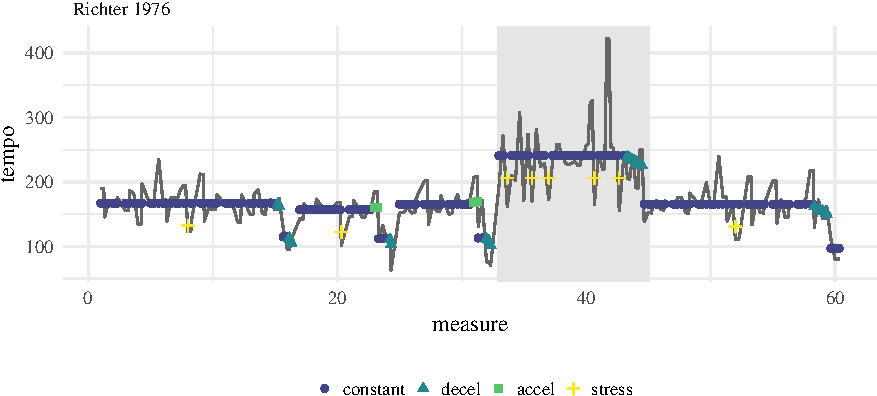
\includegraphics[width=.9\linewidth]{richter-1}
  \caption{Note-by-note tempos for a recording of Chopin's Mazurka
    Op.\ 68 No.\ 3 by Sviatislav Richter. The solid line are the
    observed tempos, while the dots represent inferred tempo states
    from our model. }
  \label{fig:richter}
\end{figure}
\autoref{fig:richter} shows the tempo\footnote{Technically, by
  ``tempo'', we mean the ratio of musical time to clock time as $0.25$
  beats $/$ $0.1$ seconds $=$ 150 beats per minute. A musician would
  likely think of ``tempo'' more broadly as something like a ``typical
  speed regime'' akin to the ``constant tempo'' state we use in our
  decision model below. We will not generally distinguish between
  these two interpretations and use the more succinct ``tempo''.}
  in beats-per-minute (b.p.m.) of
a recording made by Sviatislav Richter of Chopin's Mazurka Op.\ 68
No.\ 3. The solid line shows the actual tempo at which he plays each
note, while the colored points correspond to our model's inferences
for his actual intentions. Some of this intent is prescribed  by
Chopin in his music, but the extent to which Richter observes Chopin's
indications makes his recording different from those of other
pianists. It is these differences that we hope to capture and understand.

\subsection{Related work}
\label{sec:related-work}


 
The vast majority of work at the intersection of statistics or machine
learning and classical music analysis has focused on a handful of tasks,
most notably structure analysis, music generation, and score
alignment.

Analysis of musical structure and its relationships with interpretation
forms the basis of music theory, and hence constitutes the core of standard
conservatory curricula, along with history and performance. Automatically learning musical structures
from performances without expert input has become more relevant
recently. \citet{RenDunson2010} use Dirichlet process models to identify
similar sections of individual classical music
performances. \citet{RobertsEngel2018} use variational autoencoders to
learn long-term structure with an explicit goal toward improved
automatic music composition.

Computer music generation and composition has a long
history~\citep{SturmBen-Tal2019,Boulanger-LewandowskiBengio2012,Collins2016,Ariza2005,FlossmannGrachten2013}.
It is actively investigated, especially using deep
learning~\citep{HadjeresPachet2017}, and has become commercially
relevant for advertising and video games through companies like
Aiva (\url{aiva.ai}), and Melodrive (\url{melodrive.com}). Google has
developed the Magenta project to enable open-source music
composition~\citep{RobertsHawthorne2018}.

The score alignment
problem matches live or recorded performances to the musical score, a necessary
processing step for any type of automated analysis. On-line alignment processes
audio waveforms in real-time 
and is sometimes called score
following~\citep{DannenbergRaphael2006,Cont2010,ContSchwarz2007,ArztWidmer2015}. Audio
matched to the score can then be used as an input for automated
musical accompaniment~\citep{Raphael2010,Vercoe1985,Dannenberg1985}.
Given recorded accompaniment, these systems seek to
modulate playback in response to a live soloist who both makes
interpretive timing decisions and mistakes. Off-line alignment~\citep{Earis2007} can be
used for simply analyzing the recordings, as we do here, or for
generating features that describe the
performance~\citep{ThickstunHarchaoui2017}, possibly for later analysis
in recommender
systems~\citep{McFeeLanckriet2011,OordDieleman2013}. For an overview
of these and related goals in music information retrieval, see~\citet{schedl2014music}.

\subsection{Our contributions}
\label{sec:our-contributions}

In this paper, we develop a switching Kalman filter model for the
tempo decisions a performer makes in recorded classical music. We
present an algorithm for performing likelihood inference, estimate our
model using a large collection of recordings of the same composition,
and demonstrate how the model is able to recover performer intentions,
and how they relate to standard musical analysis. We use the learned
low-dimensional representations to compare and contrast the recordings
of different recordings through hierarchical clustering, and 
discuss how this analysis facilitates more informed musical
comparisons of the recordings.

In \autoref{sec:materials-methods} we discuss our dataset, a
collection of professional recordings of Chopin's Mazurka Op.\ 68 No.\
3. We also present our model for tempo decisions, discuss it's
statistical estimation, and detail its utility for understanding
interpretations as a musician would. \autoref{sec:analys-chop-mazurka}
presents a music theory interpretation of the Mazurka. We discuss how
different performers approach this piece through the lens of our model.
We also examine a clustering based on our model and interpret the musical
meaning of these clusters.  Finally, we contrast our approach with
some alternative non-parametric
smoothers, discusses their deficiencies relative our switching model,
and examine some issues with our proposal.




\section{Materials and methods}
\label{sec:materials-methods}




%\subsection{Data and preprocessing}

In this paper, we examine note-by-note tempos for 46 recordings of
Chopin's Mazurka Op.\ 68, No.3. The data are part of a large
collection of the complete Chopin Mazurkas and other recordings
collected and analyzed by the Center for the History and Analysis of
Recorded Music (CHARM) in the United Kingdom~\citep{CHARM-site}. The
recordings were processed using the note-onset detection algorithm
developed in~\citep{Earis2007} and are available for
download~\citep{Earis2009}. We use the data for ``all rhythmic
events'', which includes the time of each note attack as well as it's
relative loudness.
%For the sake of reproducibility, we have included this data in our R package.

\subsection{Switching state-space models}

State-space models define the probability distribution of a continuous
time series $Y$ by reference to some imagined, continuous hidden state, $X$. In
particular, the observation at time $i$ is assumed to be
independent of past and future observations conditional on the state
at time $i$. Coupling with temporal dependence for $X$---most
frequently obeying the Markov property---induces a temporal model for
the observations.  The most general form of a state-space model is
then characterized by the 
measurement equation (the conditional probability of observations
given the states),
the transition equation (specifying the nature of Markovian
dynamics), and an initial distribution for the state: 
\begin{equation}
\begin{aligned}
  y_i &= f_\theta(x_i,\epsilon_i), &
  x_{i+1} &= g_\theta(x_i,\eta_i), &
  x_1 &\sim F,
\end{aligned}
\label{eq:ssmod}
\end{equation}
where $\epsilon_i$ are $\eta_i$ are marginally independent and
identically distributed  as well as mutually independent. Both
$y_i$ and $x_i$ can be vector-valued, though in our
application, $y_i$ will be univariate. The
vector $\{y_i\}_{i=1}^n$ is observed, and the goal is to make
inferences for the unobserved states $\{x_i\}_{i=1}^n$ as well as any
unknown parameters $\theta$ characterizing $f_\theta$, $g_\theta$, and
the distributions of $\epsilon_i$ and $\eta_i$.
% \autoref{fig:ssmod}
% shows a directed acyclic graph for the dependence structure in the
% typical state-space model.

% \begin{figure}
%   \centering
%   % The continuous state vector is represented by a circle.
%   % "minimum size" makes sure all circles have the same size
%   % independently of their contents.
%   \begin{tikzpicture}[>=latex,text height=1.5ex,text
%     depth=0.25ex,ampersand replacement=\&] 
%     \matrix[row sep=1cm,column sep=1cm] {
%       % first line: hidden continuous state
%       \node (x_k-2) {$\cdots$}; \&
%       \node (x_k-1) [state] {$\mathbf{x}_{i-1}$}; \&
%       \node (x_k)   [state] {$\mathbf{x}_i$};     \&
%       \node (x_k+1) [state] {$\mathbf{x}_{i+1}$}; \&
%       \node (x_k+2) {$\cdots$};
%       \\
%       % Second line: Measurement
%       \node (y_k-2) {$\cdots$}; \&        
%       \node (y_k-1) [measurement] {$\mathbf{y}_{i-1}$}; \&
%       \node (y_k)   [measurement] {$\mathbf{y}_i$};     \&
%       \node (y_k+1) [measurement] {$\mathbf{y}_{i+1}$}; \&
%       \node (y_k+2) {$\cdots$};
%       \\
%     };
%     % The diagram elements are now connected through arrows:
%     \path[->]
%     (x_k-2) edge (x_k-1)
%     (x_k-1) edge (x_k)	
%     (x_k)   edge (x_k+1)	
%     (x_k+1)   edge (x_k+2)	
%     (x_k-1) edge (y_k-1)
%     (x_k) edge (y_k)
%     (x_k+1)   edge (y_k+1);
%   \end{tikzpicture}
%   \caption{State-space model. Filled objects are observed, circles
%     indicate that both hidden and observed states are
%     continuous.\label{fig:ssmod}} 
% \end{figure}

If $f_\theta$ and $g_\theta$ are linear with $\epsilon_i$ and
$\eta_i$ normally distributed, Equation \eqref{eq:ssmod} becomes
\begin{equation}
  \begin{aligned}
    x_{i+1}&= d+T x_i + \eta_{i}, 
    & \eta_i &\sim N(0,\ Q),     
    &x_1 &\sim N(x_0,\ P_0),\\
    y_i&= c + Z x_i + \epsilon_i,     
    & \epsilon_i &\sim N(0,\ G), \\
  \end{aligned}
  \label{eq:lgmod}
\end{equation}
where the matrices $d,\ T,\ c,\ Z,\ Q,$ and $G$ are allowed to depend
on $\theta$ and can potentially vary (deterministically) with $i$. In this case,
the Kalman filter, %\autoref{alg:kalman}
\citep[see e.g.,][]{Kalman1960,Harvey1990},
provides closed form 
solutions for the conditional
distributions of the states and gives the likelihood of $\theta$
given data. For completeness, we have included the Kalman filter in
the Supplementary Material.% as \autoref{alg:kalman}.
% \begin{algorithm}[t!]
%   \begin{singlespace}
%   \caption{Kalman filter: estimate $x_i$ conditional on
%     $\{y_j\}_{j=1}^i$, for all $i=1,\ldots,n$ and calculate the log likelihood
%     for $\theta$\label{alg:kalman}}
%   \begin{algorithmic}
%     \STATE {\bf Input:} $Y$, $x_0$, $P_0$, $d,\ T,\ c,\ Z,$ and $G$
%     \STATE $\ell(\theta) \leftarrow 0$ \COMMENT{Initialize the log-likelihood}
%     \FOR{$i=1$ to  $n$}
%     \STATE $\begin{aligned}\varx_{i}
%       &\leftarrow d + T x_{i-1|i-1}, & P_i &\leftarrow Q + T P_{i-1|i-1}
%       T^\top\end{aligned}$ \COMMENT{Predict current state}
%     \STATE $\begin{aligned}\widetilde{y}_i
%       &\leftarrow c + Z \varx_i, & F_i &\leftarrow G + Z P_i
%       Z^\top\end{aligned}$ \COMMENT{Predict current observation}
%     \STATE $\begin{aligned}v_i&\leftarrow y_i-\widetilde{y}_i& K_i&
%       \leftarrow P_i Z^\top F^{-1}\end{aligned}$ \COMMENT{Forecast error and 
%     Kalman gain}
%     \STATE $\begin{aligned} x_{i|i}
%       &\leftarrow \varx_i + K_i v_i, & P_{i|i} &\leftarrow P_i - P_iZ^\top
%       K_i\end{aligned}$ \COMMENT{Update}
%     \STATE $\ell(\theta) = \ell(\theta) -v_i^\top F^{-1}v_i - \log(|F_i|)$
%     \ENDFOR
%     \RETURN $\widetilde{Y}=\{\widetilde{y}_i\}_{i=1}^n,\ \varx=\{\varx_i\}_{i=1}^n,\
%     \widetilde{X}=\{x_{i|i}\}_{i=1}^n,\ P=\{P_i\}_{i=1}^n,\
%     \widetilde{P}=\{P_{i|i}\}_{i=1}^n,\ \ell(\theta)$
%   \end{algorithmic}
% \end{singlespace}
% \end{algorithm}

% However, in many applications, researchers are not so
% lucky. For nonlinear  or non-Gaussian models, approximate solutions
% exist using the particle filter and its derivatives (see for
% example~\citet{Kitagawa1987,Kitagawa1996}
% and~\citet{DoucetDe-Freitas2001} for an exposition of the particle
% filter and~\citet{KoyamaPerez-Bolde2010}
% and~\citet{DejongDharmarajan2009a} for improvements).

While the Kalman filter %\autoref{alg:kalman}
returns the likelihood for $\theta$, 
inference for the the mean and variance
of $X$ is conditional only on the preceding observations
$\{y_j\}_{j=1}^i$: $\varx_i=\Expect{x_i\given y_1\ldots,y_i}$ and
$P_i=\Var{x_i\given y_1,\ldots,y_i}$. To
incorporate all future observations into these estimates, the Kalman
smoother is required.
% \begin{algorithm}[t!]
%   \begin{singlespace}
%   \caption{Kalman smoother (Rauch-Tung-Striebel): estimate $\hat{X}$ conditional on
%     $Y$\label{alg:kalman-smoother}} 
%   \begin{algorithmic}
%     \STATE {\bf Input:} $\varx$, $\widetilde{X}$, $P$, $\widetilde{P}$,
%     $T,$ $c$, $Z$.
%     \STATE $t=n$,
%     \STATE $\hat{x}_{n}\leftarrow \widetilde{x}_n$, 
%     \WHILE{$t>1$}
%     \STATE $\hat{y}_i \leftarrow c + Z\hat{x}_i,$
%     \COMMENT{Predict observation vector}
%     \STATE $\begin{aligned} e &\leftarrow \hat{x}_i -
%       \varx_i, & V &\leftarrow P_i^{-1}\end{aligned}$,
%     \STATE $t\leftarrow i-1$, \COMMENT{Increment}
%     \STATE $\hat{x}_i = \widetilde{x}_i + \widetilde{P}_i T Ve $ 
%     \ENDWHILE
%     \RETURN $\widehat{Y}=\{\hat{y}_i\}_{i=1}^n, \hat{X}=\{\hat{x}_i\}_{i=1}^n$
%   \end{algorithmic}
% \end{singlespace}
% \end{algorithm}
There are many different smoother algorithms tailored for different
applications. %\autoref{alg:kalman-smoother} (Supplementary Material),
The smoother we use, due
to~\citet{RauchStriebel1965}, is often referred to as the classical
fixed-interval smoother~\citep{AndersonMoore1979}. It produces only
the unconditional expectations of the hidden state
$\hat{x}_i=\Expect{x_i\given y_1,\ldots,y_n}$ for the sake of
computational speed. This version is more appropriate for inference in
the type of switching models we discuss below. We again provide this
algorithm in the Supplementary Material.


Linear Gaussian state-space models can be made quite flexible
by expanding the state vector or allowing the parameter matrices to
vary with time. Furthermore, this general form encompasses many
standard time series models: ARIMA models, ARCH and GARCH models,
stochastic volatility models, exponential smoothers, and
more~\citep[see][for many other
examples]{DurbinKoopman2001}. Nonlinear, non-Gaussian versions have
been extensively
studied~\citep{DurbinKoopman1997,Fuh2006,Kitagawa1987,Kitagawa1996}
and algorithms for filtering, smoothing, and parameter estimation have
been derived~\citep[e.g.,][]{KoyamaPerez-Bolde2010,AndrieuDoucet2010}. 
However, these models are less useful
for change-point detection or other forms of discontinuous behavior
when the times of discontinuity are unknown. 

To remedy this deficiency, one can use a switching state-space
model as shown in \autoref{fig:switchss}. Here, we assume $S$ is a
hidden, discrete process with Markovian dynamics. Then, the value of
the hidden state at time $i$, $s_i=k$ say, can determine the evolution of
the continuous model at time $i$. The graphical model in
\autoref{fig:switchss} gives the conditional independence properties
we will use in our model for musical interpretation, but this
represents just one of many possibilities. Switching state-space models have a long
history with many applications from
economics~\citep{KimNelson1998,Kim1994,Hamilton2011} to speech
processing~\citep{FoxSudderth2011} to animal
movement~\citep{PattersonThomas2008,BlockJonsen2011}. An excellent
overview of the history, typography, and algorithmic developments can
be found in~\citep{GhahramaniHinton2000}. In Equation~\eqref{eq:lgmod}, the
parameter matrices were not time varying. In our switching model, we
allow the switch states $s_i, s_{i-1}$, along with the parameter
vector $\theta$, to determine the specific dynamics at time $i$:
\begin{equation}
  \begin{aligned}
    x_1 &\sim N(x_0,\ P_0),\\
    x_{i+1}&= d(s_i,s_{i-1})+T(s_i,s_{i-1}) x_i + \eta_i, 
    & \eta_i &\sim N(0,Q(s_i,s_{i-1})),\\
    y_i&= c(s_i) + Z(s_i) x_i + \epsilon_i, & \epsilon_i &\sim N(0, G(s_i)).
  \end{aligned}
\end{equation}
In other words, the hidden Markov (switch) state determines which parameter
matrices govern the evolution of the system. 






\begin{figure}
  \centering
  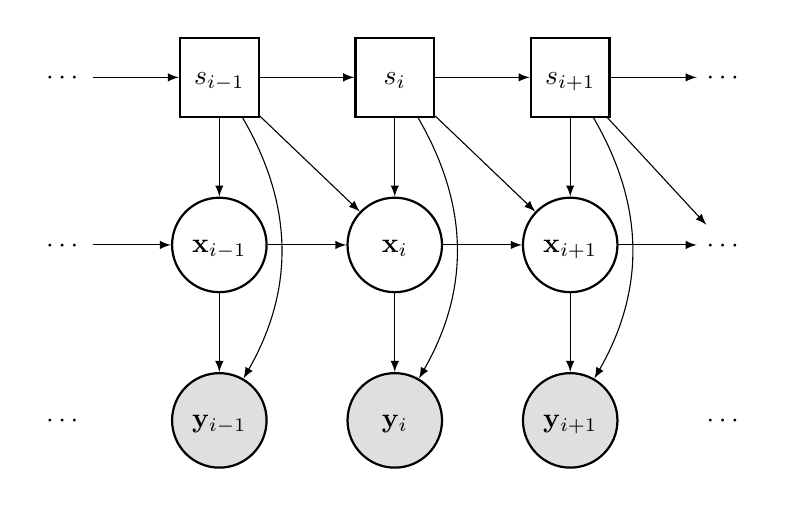
\begin{tikzpicture}[>=latex,text height=1.5ex,text depth=0.25ex,ampersand replacement=\&]
    % The various elements are conveniently placed using a matrix:
    \matrix[row sep=1cm,column sep=1cm] {
      % First line: Switch state
      \node (s_k-2)  {$\cdots$}; \&
      \node (s_k-1) [switch]{$s_{i-1}$}; \&
      \node (s_k)   [switch]{$s_i$};     \&
      \node (s_k+1) [switch]{$s_{i+1}$}; \&
      \node (s_k+2) {$\cdots$};
      \\
      % Second line: hidden continuous state
      \node (x_k-2) {$\cdots$}; \&
      \node (x_k-1) [state] {$\mathbf{x}_{i-1}$}; \&
      \node (x_k)   [state] {$\mathbf{x}_i$};     \&
      \node (x_k+1) [state] {$\mathbf{x}_{i+1}$}; \&
      \node (x_k+2) {$\cdots$};
      \\
      % Third line: Measurement
      \node (y_k-2) {$\cdots$}; \&        
      \node (y_k-1) [measurement] {$\mathbf{y}_{i-1}$}; \&
      \node (y_k)   [measurement] {$\mathbf{y}_i$};     \&
      \node (y_k+1) [measurement] {$\mathbf{y}_{i+1}$}; \&
      \node (y_k+2) {$\cdots$};
      \\
    };
    % The diagram elements are now connected through arrows:
    \path[->]
    (s_k-2) edge (s_k-1)
    (s_k-1) edge (s_k)	
    (s_k)   edge (s_k+1)	
    (s_k+1)   edge (s_k+2)	
    
    (x_k-2) edge (x_k-1)
    (x_k-1) edge (x_k)	
    (x_k)   edge (x_k+1)	
    (x_k+1)   edge (x_k+2)	
    
    (s_k-1) edge (x_k-1)
    (s_k) edge (x_k)
    (s_k+1)   edge (x_k+1)
    
    (x_k-1) edge (y_k-1)
    (x_k) edge (y_k)
    (x_k+1)   edge (y_k+1)
    
    (s_k-1) edge (x_k)
    (s_k) edge (x_k+1)
    (s_k+1)   edge (x_k+2)
    
    (s_k-1) edge[bend left] (y_k-1)
    (s_k) edge[bend left] (y_k)
    (s_k+1)   edge[bend left] (y_k+1)
    ;
  \end{tikzpicture}
  \caption{Switching state space model. Filled objects are observed,
    rectangles are discrete, and circles are continuous.\label{fig:switchss}}
\end{figure}






\subsection{A model for tempo decisions}


In musical scores, {\em tempi} (the Italian plural of tempo) may be
marked at various points throughout a piece of music. The
beginning can be either explicit, with a metronome marking to
indicate the number of beats per minute (b.p.m.), and/or with some words
(e.g., {\em Adagio}, {\em Presto}, {\em Langsam}, Sprightly) which indicate an
approximate speed. 
\begin{figure}[t!]
  \centering
  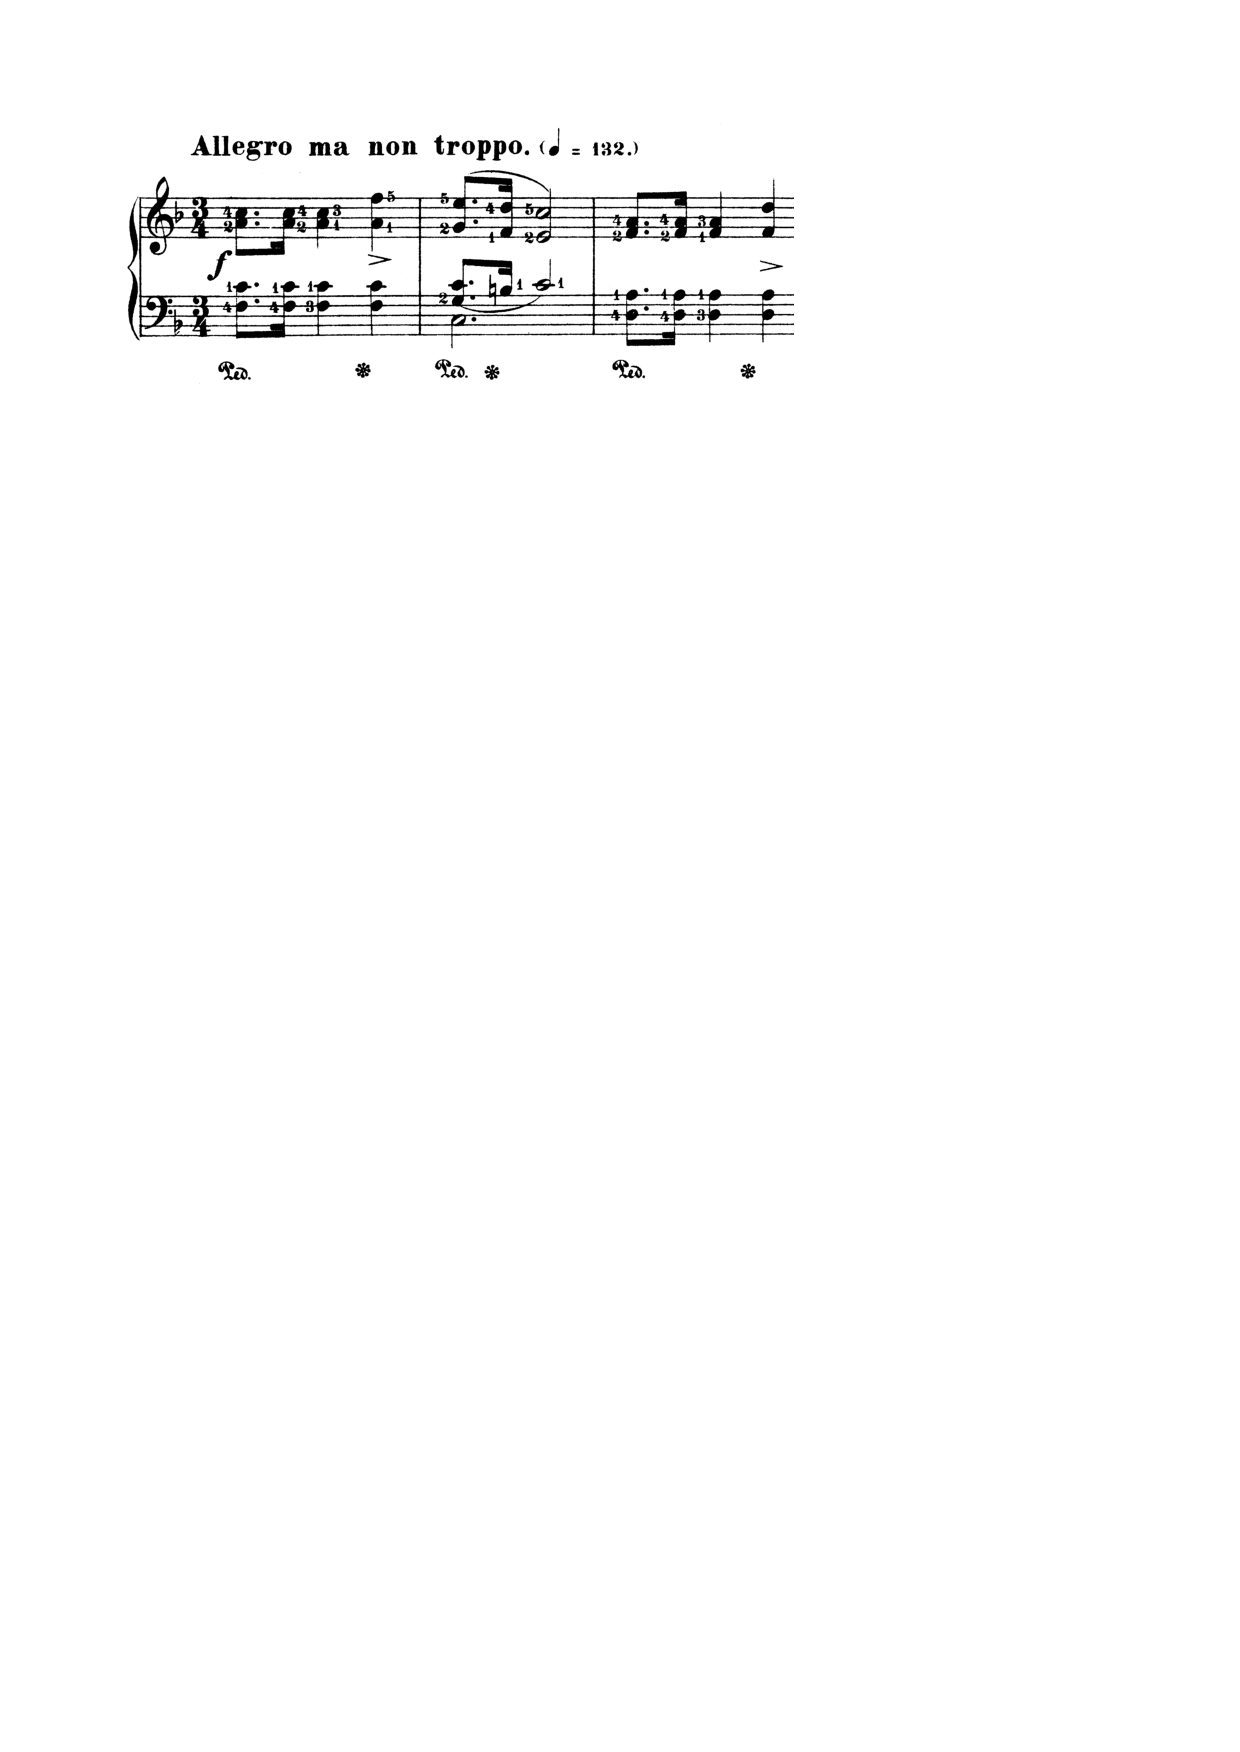
\includegraphics[height=3cm]{mazurka-top.pdf}
  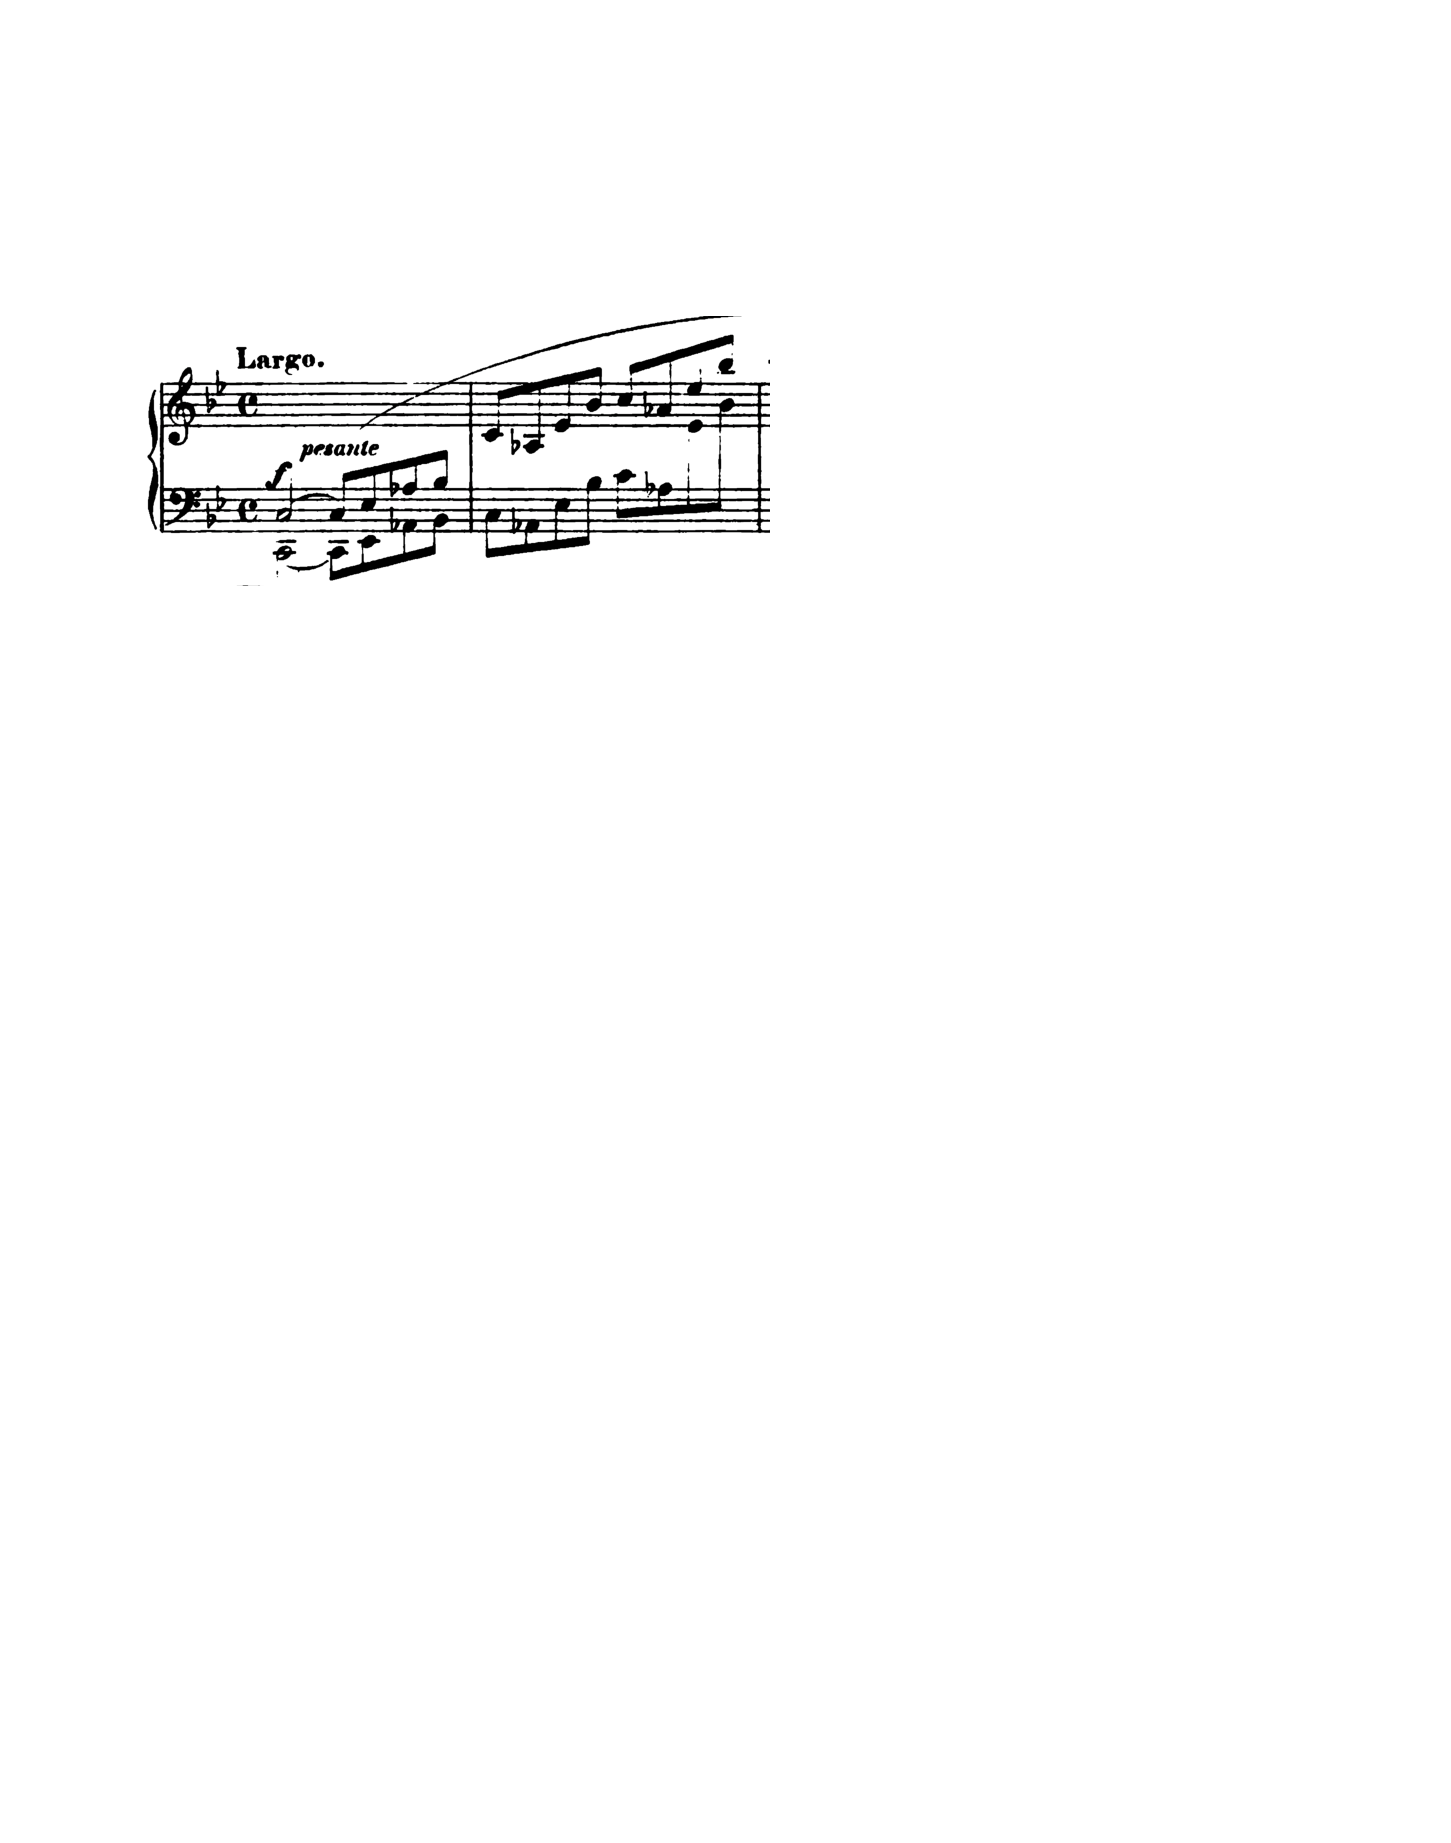
\includegraphics[height=3cm]{ballade-top.pdf}
  \caption{The beginning of two Chopin piano compositions: the Mazurka
    we analyze is on the left while the Ballade No.\ 1, Op.\ 23 is on
    the right.}
  \label{fig:tempo-markings}
\end{figure}
\autoref{fig:tempo-markings} shows the beginning of two Chopin piano
compositions: the Mazurka we analyze and the Ballade No.\ 1, Op.\
23. The initial tempo of the Mazurka is given with a metronome
marking as well as the Italian phrase {\em Allegro ma non troppo}
(``cheerful, but not too much''). The beginning of the Ballade is 
marked {\em Largo}, which translates literally as ``broad'' or
``wide'', and modified by the stylistic indication {\em pesante}
(``heavy''). Obviously, the metronome markings are much more exact,
though even these are often viewed as suggestions rather than
commandments. The metronome markings in most of Beethoven's
compositions, for example, are notoriously fast, and some scholars
believe that his metronome (one of the first ever made) was
inaccurate~\citep{ForsenGray2013}. Often, compositions will have numerous such markings later
in the piece of music, but these are only some of the ways that tempo
is indicated. Composers will also indicate periods of speeding-up
(\emph{accelerando}) or
slowing-down (\emph{ritardando}).

Absent instructions from the composer, performers generally maintain
(or try to maintain) a steady tempo, and this assumption plays a major
role in our model of tempo decisions. Of course, a normal human 
never plays precisely like a 
metronome, although she may try quite hard to do so. The observed
ratio of musical time to clock time
is therefore best viewed as stochastic, the sum of an
intentional, constant tempo, plus noise representing inaccuracy
or, perhaps more charitably, unintentional variation which the
listener fails to perceive as ``wrong''. For instance, the example in
\autoref{fig:short-perf} shows the beginning of the piece as performed
by Arthur Rubinstein in a 1961 recording. 
\begin{figure}[t!]
 \centering
 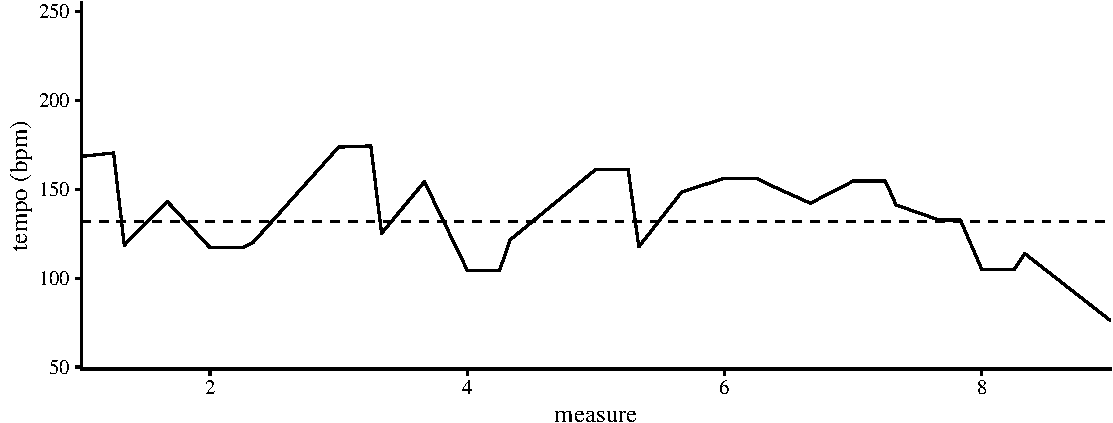
\includegraphics[width=.9\linewidth]{small-rubinstein-1961-1}
 \caption{The solid line shows the observed note-by-note tempo for
   the beginning of the Mazurka as performed by Arthur Rubinstein in
   1961. The dashed line indicates 132 b.p.m.}
 \label{fig:short-perf}
\end{figure}
The solid line shows the
actual, performed tempo, while the dashed horizontal line is placed at
the indicated tempo of 132 b.p.m. The figure has three important
lessons: (1) observed speed varies around intended tempo; (2) 132 b.p.m.\ is
not necessarily the tempo a performer will choose despite the
indication; and (3) performers have other tempo intentions which are
not marked, like the pronounced slow-down in measures 7--8.

Estimating intended {\em tempi} would be reasonably simple, perhaps, 
if the locations of the tempo changes were known. In such a case,
the average of tempi between changes may be a good estimate as
could the slope of known speed-ups or slow-downs. However, performers
take liberties with these decisions, exactly the liberties we would
like to discover. This suggests employing a switching model with a
small number of discrete states.

Similar to~\citet{GuRaphael2012}, we propose a Markov model for $S$ on four
states for four different performance behaviors
with transition probability
diagram given by \autoref{fig:transmat}.
\begin{figure}[tb!]
  \centering
  \tikzstyle{switch}=[rectangle,
  thick, minimum size=1cm, draw=black]
  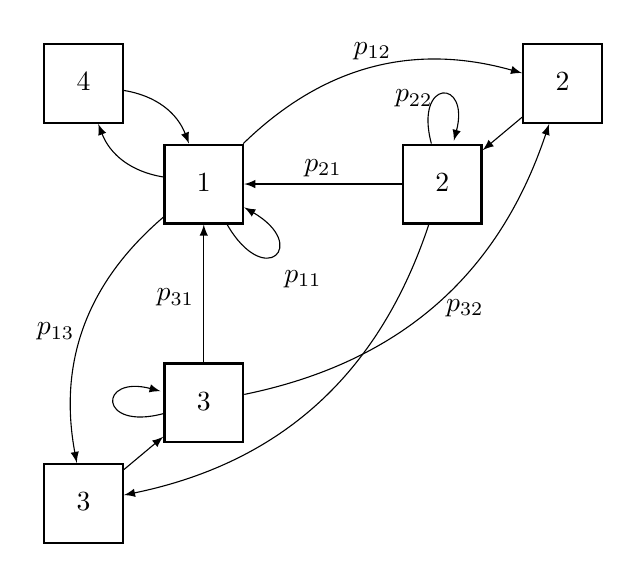
\begin{tikzpicture}[>=latex,text height=1.5ex,text depth=0.25ex]
    \matrix[row sep=0.25cm,column sep=.5cm] {
      \node (S4) [switch] {$4$}; &&&&& & \node (S22) [switch] {$2$};\\
      &\node (S1) [switch] {$1$}; &&&& \node (S2) [switch] {$2$}; \\
      \\ \\ \\ \\ \\ \\
      &\node (S3) [switch] {$3$};\\
      \node (S33) [switch] {$3$};\\
    };
    \path[->]
    (S1) edge [bend left]  (S4)
    (S4) edge [bend left] (S1)
    (S1) edge [bend left] node [above] {$p_{12}$}(S22)
    (S22) edge (S2)
    (S2) edge [bend left] (S33)
    (S1) edge [bend right] node [left] {$p_{13}$}(S33)
    (S33) edge (S3)
    (S3) edge [bend right] node [right] {$p_{32}$}(S22)
    (S3) edge [loop left](S3)
    (S2) edge [loop above] node [left] {$p_{22}$}(S2)
    (S3) edge node [left] {$p_{31}$}(S1)
    (S2) edge node [above] {$p_{21}$}(S1);
   \path[->] (S1) edge [out=300,in=330,looseness=8] node [below right]
   {$p_{11}$} (S1);
  \end{tikzpicture}
  \caption{Transition diagram. The four states are: constant tempo
    (1), deceleration (2), acceleration (3), and emphasis (4).\label{fig:transmat}}
\end{figure}
The 4 switch states correspond to 4 different behaviors for the
performer: (1) constant tempo, (2) speeding up, (3) slowing down, and
(4) single note stress. As shown in the diagram, we only allow certain
transitions for musical reasons and for estimability. The marked
transition probabilities are sufficient to infer the remainder. The fourth
state, stress, corresponds to {\em tenuto}, a common feature of
musical performance. Such stresses may be marked with a line over the
note in question, but are more often a feature of the performer taste,
corresponding to a longer-than-written duration of a particular
note. Such emphases occur for a variety of musical purposes---emphasis
of the beat in running notes, the top of a
phrase, a ``landing point'' where a phrase ends, etc.---but are always
within the frame of constant tempo. Thus we allow stress to occur only
after and before notes in state 1. Furthermore, we cannot allow
state 2 or state 3 to return immediately to state 1, or else ``stress'' could
happen through these pathways. We impose related constraints for a transition from state 2
to state 3 and vice versa. Essentially, transitions into these states must remain
there before leaving. Thus, the entire transition diagram is
fully determined. This process can  be viewed equivalently as a
second-order Markov chain.
% We discuss some potential improvements at the end
% of~\autoref{sec:analys-chop-mazurka}. 


Our data gives $y_i$ as the observed tempo (in b.p.m.) of the note (or
chord) of the $i^{th}$ note onset in Chopin's Mazurka Op.\ 68 No.\ 3. The
hidden continuous variable ($X_i$) is 
taken to be a two component vector with the first component being the
prevailing tempo and the second the amount of acceleration. The amount, or
existence, of acceleration is determined by the current and previous
switch states. We use $l_i$ to denote the musical duration of
a particular note as given by the written score, so, throughout this piece, a quarter-note (\quarternote) has $l_i=1/3$, an
eighth note (\eighthnote) has $l_i=1/6$, etc. This is because each
measure contains three quarter notes. In more complicated
music with changing time signatures or instances where the notation
doesn't necessarily correspond with the time signature, more care
would be required. The observed tempo is already normalized to account
for variable note durations, but the intentional tempo and its
variance should be proportional to $l_i$. When the performer is in state 1 (or
transits in and out of state 4), we take the prevailing tempo as
constant with no acceleration: $X_{i+1} = X_i$. 
Corresponding to these configurations, the parameter
matrices are given in \autoref{tab:parmats} (transition equation) and
\autoref{tab:parmats2} (measurement equation).
\begin{table}
\centering
\begin{tabular}[h!]{@{}llcccc@{}}
\toprule
%&&&\multicolumn{3}{c}{Transition equation}\\
  \multicolumn{2}{c}{Switch states} &\phantom{a}& \multicolumn{3}{c}{parameter
                                      matrices}\\
  \cmidrule{1-2} \cmidrule{4-6}
  $s_i$ & $s_{i-1}$ && $d$ & $T$ & $Q$ \\
  \midrule
  $1$ &  $1$ && 0 & $\begin{pmatrix}1&0\\0&0\end{pmatrix}$ 
                 & $\begin{pmatrix}0&0\\0&0\end{pmatrix}$\\
  $2$ & $1$ && $\begin{pmatrix} l_i\mu_{\textrm{acc}}\\ \mu_{\textrm{acc}}\end{pmatrix}$ 
                                    & $\begin{pmatrix} 1 & 0 \\ 0 &
                                      0 \end{pmatrix}$ 
        & $\sigma_{\textrm{acc}}^2\begin{pmatrix} l_i^2 & l_i\\ l_i & 1 \end{pmatrix}$\\
  $3$ & $1$ && $\begin{pmatrix} -l_i\mu_{\textrm{acc}}\\ -\mu_{\textrm{acc}}\end{pmatrix}$ 
                                    & $\begin{pmatrix} 1 & 0 \\ 0 &
                                      0 \end{pmatrix}$ 
        & $\sigma_{\textrm{acc}}^2\begin{pmatrix} l_i^2 & l_i\\ l_i & 1 \end{pmatrix}$\\
  $4$ & $1$ && $\begin{pmatrix}0\\\mu_{\textrm{stress}}\end{pmatrix}$ 
                                     & $\begin{pmatrix}1&0\\0&0\end{pmatrix}$
          & $\begin{pmatrix}0&0\\0&\sigma_{\textrm{stress}}^2\end{pmatrix}$\\
  $2$ & $2$ && 0 & $\begin{pmatrix} 1 & l_i \\ 0 & 1 \end{pmatrix}$ 
        & $\begin{pmatrix}0&0\\0&0\end{pmatrix}$\\
  $3$ & $2$ && $\begin{pmatrix} -l_i\mu_{\textrm{acc}}\\ -\mu_{\textrm{acc}}\end{pmatrix}$ 
                                    & $\begin{pmatrix} 1 & 0 \\ 0 &
                                      0 \end{pmatrix}$ 
        & $\sigma_{\textrm{acc}}^2\begin{pmatrix} l_i^2 & l_i\\ l_i & 1 \end{pmatrix}$\\
  $1$ & $2$ && $\begin{pmatrix} \mu_{\textrm{tempo}}\\0\end{pmatrix}$ & 0
        & $\begin{pmatrix} \sigma^2_{\textrm{tempo}} & 0\\ 0 & 0 \end{pmatrix}$\\
  $3$ & $3$ && 0& $\begin{pmatrix} 1 & l_i \\ 0 & 1 \end{pmatrix}$ 
        & $\begin{pmatrix}0&0\\0&0\end{pmatrix}$\\
$2$ & $3$ && $\begin{pmatrix} l_i\mu_{\textrm{acc}}\\ \mu_{\textrm{acc}}\end{pmatrix}$ 
                                    & $\begin{pmatrix} 1 & 0 \\ 0 &
                                      0 \end{pmatrix}$ 
        & $\sigma_{\textrm{acc}}^2\begin{pmatrix} l_i^2 & l_i\\ l_i & 1 \end{pmatrix}$\\
  $1$ & $3$ && $\begin{pmatrix} \mu_{\textrm{tempo}}\\0\end{pmatrix}$ & 0
          & $\begin{pmatrix} \sigma^2_{\textrm{tempo}} & 0\\ 0 & 0 \end{pmatrix}$\\
  $1$ &  $4$ && 0 & $\begin{pmatrix}1&0\\0&0\end{pmatrix}$ 
        & $\begin{pmatrix}0&0\\0&0\end{pmatrix}$\\
  \bottomrule
\end{tabular}
\caption{Parameter matrices of the transition equation for the switching state space model.\label{tab:parmats}}
\end{table}
%
%
\begin{table}
\centering
\begin{tabular}[h!]{@{}llcccc@{}}
\toprule
%&&&\multicolumn{3}{c}{Measurement equation}\\
  \multicolumn{2}{c}{Switch states} &\phantom{a}& \multicolumn{3}{c}{parameter
                                                    matrices}\\
  \cmidrule{1-2} \cmidrule{4-6}
  $s_i$ &&& $c$ & $Z$ & $G$\\
  \midrule
  $4$ & && 0 & $\begin{pmatrix} 1 & 1 \end{pmatrix}$ &
                                                                  $\sigma^2_\epsilon$\\
  else &&& 0 & $\begin{pmatrix} 1 & 0 \end{pmatrix}$ &
                                                                  $\sigma^2_\epsilon$\\
\bottomrule
\end{tabular}
\caption{Parameter matrices of the measurement equation for the switching state space model.\label{tab:parmats2}}
\end{table}
So for any performance, we want to be able to estimate
the following parameters: $\sigma_{\textrm{tempo}}^2$, $\sigma_{\textrm{acc}}^2$, $\sigma^2_{\textrm{stress}}$,
$\sigma_\epsilon^2$, the probabilities of the transition matrix (there
are 7), and means $\mu_{\textrm{tempo}}$, $\mu_{\textrm{acc}}$, and $\mu_{\textrm{stress}}$. Lastly, we have the initial state distribution
\[
x_1\sim N\left( \begin{pmatrix}\mu_1\\0\end{pmatrix}
  ,\ \begin{pmatrix} \sigma^2_1 & 0\\0 & 0
  \end{pmatrix}\right)\; \; \textrm{where} \; \; s_1=1.
\]

To clarify this model, we explicate two different behaviors: discrete
sequence $1\rightarrow 4\rightarrow 1$ (emphasis within constant tempo) and discrete sequence
$1\rightarrow 1\rightarrow 2$ (constant tempo to slowing down). In the
first case, the state space system has the following configurations
{\footnotesize
\begin{align*}
  1\rightarrow 4 && 4\rightarrow 1\\
  x_{2} &= \begin{pmatrix} 0\\ \mu_{\textrm{stress}} \end{pmatrix}
  + \begin{pmatrix}1&0\\0&0\end{pmatrix} x_{1} +
                           \mbox{N}\left(0,\ \begin{pmatrix}0&0\\0&\sigma_{\textrm{stress}}^2\end{pmatrix}\right)
        &   x_{3}
                    &= 
  \begin{pmatrix}1&0\\0&0\end{pmatrix} x_{2} \\
  y_2 &= (1\quad  1)  x_2 + \mbox{N}(0,\
                                 \sigma_\epsilon^2) &
y_3 &= (1\quad  0) x_3 + \mbox{N}(0,\
                                 \sigma_\epsilon^2),
\end{align*}
}%
while in the second
{\footnotesize
\begin{align*}
  1\rightarrow 1 && 1\rightarrow 2\\
  x_{2} &= 
  \begin{pmatrix}1&0\\0&0\end{pmatrix} x_{1} 
        &   x_{3}
                    &= \begin{pmatrix} l_i\mu_{\textrm{acc}}\\ \mu_{\textrm{acc}}\end{pmatrix} +
  \begin{pmatrix}1&0\\0&0\end{pmatrix} x_{1} +
                         \mbox{N}\left(0,\ \sigma_{\textrm{acc}}^2\begin{pmatrix} l_i^2 & l_i\\ l_i & 1 \end{pmatrix}\right)\\
  y_2 &= (1\quad  0)  x_2 + \mbox{N}(0,\
                                 \sigma_\epsilon^2) &
y_3 &= (1\quad  0) x_3 + \mbox{N}(0,\
                                 \sigma_\epsilon^2).
\end{align*}
}%
Recall that in any case $y_i$ is a scalar and $x_i \in \mathbb{R}^2$.


\subsection{Estimation and computational issues}
\label{sec:computational-issues}

To understand the performance decisions of individual musicians, we
wish to simultaneously learn $\theta$, $S$, and $X$. Because the
switch states $S$ and the continuous states $X$ are both hidden, this becomes
an NP-hard problem. In particular, there are $4^n$ possible paths
through the switch variables, so evaluating the likelihood to maximize
over $\theta$ via the Kalman filter at each path is intractable. 
\citet{GhahramaniHinton2000} give a variational approximation to
estimate $\theta$ without also estimating $S$, but, as our goal is to
learn both, we use the particle filtering approximation described by
\citet{FearnheadClifford2003}. ~\cite{WhiteleyAndrieu2010} refer to
this algorithm as the Discrete Particle Filter, and it can be seen as
an instance of the ``Beam Search'' optimization
technique~\citep{Bisiani1992}. The details are given in
\autoref{alg:dpf} but the intuition is as follows: (1) for the first
few time points, evaluate
one step of the Kalman filter for each possible subsequent discrete
state and store all these values; (2) calculate weights for each path
by updating previous weights with the likelihood multiplied by the transition probability;
(3) continue through time until the number of stored values exceeds
some threshold storage limit; (4) from that point forward, subselect
the ``best'' paths using a sampling scheme.
\begin{algorithm}[t!]
  \caption{Discrete particle filter\label{alg:dpf}}
  \begin{algorithmic}[1]
  \STATE {\bfseries Input:}
  $Y$, $\theta$, $\pi_1$ probability vector over initial states
  (paths), $B$ maximum beam width
  \FOR{$i=1$ {\bfseries to} $n$}
  \STATE Set $b_i=|\{\pi_i>0\}|$, the number of current paths
  \STATE Use %\autoref{alg:kalman}
  the Kalman filter to calculate the 1-step likelihood
  $\ell_i$ for each path and every potential state $s_{i+1}$ resulting in $b_i|S|$ particles
  \STATE Set $\pi_{i+1} \leftarrow \pi_i\ell_i p_i$: multiply the path
  probability by the likelihood and the probability of
  transitioning. Normalize $\pi$.
  \STATE Set $b_{i+1}=|\{\pi_{i+1}>0\}|$ . If $b_{i+1} > B$, resample the
  weights to get $B$ non-zero weights and renormalize
  \ENDFOR
  \STATE Return $B$ paths $\{S_b\}_{b=1}^B$ along with their weights $\pi_{n}$.
\end{algorithmic}
\end{algorithm}
These paths can be
selected greedily, retaining only the highest values to that point,
though we use the resampling procedure of
\citep{FearnheadClifford2003} which is designed to 
approximate to the full discrete distribution over paths with a subset
of support points by minimizing the mean squared
error.

\autoref{alg:dpf} returns $B$ paths along with their weights through
the discrete state $S$ for a 
particular parameter value $\theta$. One
can view this as a (approximate) distribution over paths conditional
on $\theta$. Instead, we will simply take the path with the highest
weight for inference via penalized maximum likelihood. Thus, the
likelihood of a particular parameter vector $\theta$ is evaluated by
computing the best path with \autoref{alg:dpf} and then using the best
path with the Kalman filter.%\autoref{alg:kalman}.

\subsection{Penalized maximum likelihood}
\label{sec:penal-maxim-likel}

Even without the latent discrete states, parameter estimation in
state-space models is a difficult problem, often plagued by spurious
local minima and non-identifiability. The addition of discrete states
only exacerbates this issue. However, for the present application, we
have reasonably strong prior information for many of the
parameters. The three mean parameters $\mu_{\textrm{tempo}}$,
$\mu_{\textrm{acc}}$ and $\mu_{\textrm{stress}}$ have sign
restrictions in addition to strong information about their magnitude:
average tempo should be around the indicated 132 b.p.m., the average
amount of acceleration should probably be less than the size of a
stress. We also have reasonably strong information about the
probabilities of transitioning between states: self-transitions should
be reasonably likely, long periods of speeding up are less likely than
long periods of slowing down which are less likely than long periods
in the constant tempo state. Because of this information, we use
informative priors as penalties on all the parameters we
estimate. This has the effect of introducing extra curvature to the
optimization problem as well as conforming with musical intuition. The
specific choices are shown in \autoref{tab:priors}. 
\begin{table}[t]
  \centering
  \begin{tabular}{@{}rcll@{}}
    \toprule
    Parameter & \phantom{a} & Distribution & Prior mean\\
    \midrule
    $\sigma^2_{\epsilon}$ & $\sim$ & Gamma$(40,\ 10)$ & 400 b.p.m.$^2$\\
    $\mu_{\textrm{tempo}}$ & $\sim$ & Gamma$(\overline{Y}^2/100,\ 100
                                      /\overline{Y})$ & $\overline{Y}$
                                                        b.p.m.\\
    $-\mu_{\textrm{acc}} $ & $\sim$ & Gamma$(15,\ 2/3)$ & 10 b.p.m.\\
    $-\mu_{\textrm{stress}} $ & $\sim$ & Gamma$(20,\ 2)$ & 40 b.p.m.\\
    $\sigma^2_{\textrm{tempo}} $ & $\sim$ & Gamma$(40,\ 10)$ & 400
                                                               b.p.m.$^2$\\
    $\sigma^2_{\textrm{acc}} $ & $=$ & 1 & 1 b.p.m.$^2$\\
    $\sigma^2_{\textrm{stress}} $ & $=$ & 1 & 1 b.p.m.$^2$\\
    $p_{1,\cdot}$ & $\sim$ & Dirichlet$(85,\ 5,\ 2,\ 8)$ \\
    $p_{2,\cdot}$ & $\sim$ & Dirichlet$(4,\ 10,\ 1,\ 0)$ \\
    $p_{3,\cdot}$ & $\sim$ & Dirichlet$(5,\ 3,\ 7,\ 0)$ \\
    \bottomrule
  \end{tabular}
  \caption{Informative prior distributions for the music model}
  \label{tab:priors}
\end{table}
We fix $\sigma^2_{\textrm{acc}}$ and $\sigma^2_{\textrm{stress}}$ after numerical experiments suggested
that they were poorly identified.

\subsection{Is this model reasonable?}

It is reasonable to ask whether a simple model such as this is able to
accurately represent performance practice without removing musically important
information. In a statistical sense, this question is similar to the
problem of tuning parameter selection in nonparametric
estimation. Specifically, we do not want this model to
``over-smooth'' the performance, eliminating information necessary for
listener appreciation. One way to examine such a question 
is to generate a performance using the smoothed tempos learned by
the model and compare it aurally with the original recording.
\citet{GuRaphael2012} used a model similar to ours to investigate just
this question. In one study, they surveyed nine graduate piano majors at a
major conservatory on twelve different piano excerpts. The pianists
were not meaningfully able to distinguish between the synthesized and
real recordings in the majority of experiments. Our model is more
expressive than that employed in the study, and the parameters are
estimated from data rather than calibrated. We expect that a similar
study with our model would yield similar, if not better, results.


\section{Analysis of Chopin's Mazurka Op.\ 68 No.\ 3}
\label{sec:analys-chop-mazurka}

We use the model and procedures developed above to estimate the
parameters and performance choices for all 46 recordings of Chopin's
Mazurka. Here we describe the inferences our model allows on some
representative performances, describe parametric clusters determined
by our model, contrast these with some alternative approaches to music
modelling, and discuss some difficulties we encountered. All simulations and empirical calculations were performed with
\texttt{R}~\citep{R-Core-Team2019} and C++ via \texttt{Rcpp}~\citep{Eddelbuettel2013}. Figures and tables are generated
using the \texttt{tidyverse} family of
packages~\citep{Wickham2017, Wickham2016}. Dendrograms combined with
heatmaps for the proximity matrices were created with the
\texttt{heatmaply} package~\citep{GaliliOCallaghan2017}.
% The Supplemental Materials were created
% with \texttt{knitr} and
% \texttt{rmarkdown}~\citep{Xie2019,XieAllaire2018,Xie2015}.
Most
computations were implemented in parallel on a
% the Carbonate\footnote{This research was supported in part by Lilly
%   Endowment, Inc., through its support for the Indiana University
%   Pervasive Technology Institute.}
large
memory computer cluster via
the \texttt{batchtools} package~\citep{LangBischl2017}. 

\subsection{Musical analysis}
\label{sec:musical-analysis}

Throughout his life, Fr\'ed\'eric Chopin composed dozens of Mazurkas,
of which 58 have been published. Inspired by a traditional Polish
dance, these pieces gave Chopin an idiomatic style upon which to
elaborate a wide variety of different compositional techniques, a
practice German and Italian composers had employed frequently over the previous 3
centuries~\citep{BurkholderGrout2014}. Repetition of themes, figures, or even small motives plays
a central role in both the traditional dance and Chopin's compositions
as do particular rhythmic gestures~\citep{Kallberg1996}, especially the
dotted-eighth sixteenth note pattern on the first beat of a measure. 

Chopin's Op.\ 68 Mazurkas are a set of four similar works, published
posthumously in 1855. The Op.\ 68 No.\ 3, which we analyze here, was
composed in 1830, when Chopin was 20 years old. Around this time,
Chopin, already a piano virtuoso and accomplished composer, left his
native Warsaw and settled in Paris, where we would remain until his
death in 1849.

This Mazurka has a rather simplistic ternary structure with two outer
sections and a contrasting middle (ABA). The first A section is made
up of four eight-bar phrases ($aaba$). The first phrase is echoed by the
second phrase: they are nearly identical, with the two exceptions
being that (1) the
second is marked {\em piano} (soft) rather {\em forte} (strong) and (2)
the second ends on the tonic (F major) rather than the dominant
(C major). The fourth eight-bar phrase is an exact repetition of the
second. The second A section is a repeat of the first two
eight-bar phrases of the beginning. The intervening B section is 12
bars long, divided into three four-bar groups. The first four bars are
simply a repeated interval of a perfect $5^{th}$ in the left
hand. This {\em ostinato} will continue for the whole section. The remaining
eight measures consist of a four-bar phrase in the right hand repeated twice. The second differs from the first only on the final two notes, preparing the
recapitulation of the A section.

In terms of tempi, the B section is indicated to be faster, with the
marking {\em Poco pi\`u vivo} (a little livelier). The B section ends
with a {\em ritardando} into the following A section. The $b$ section ends
with a {\em fermata} in measure 24, indicating an arbitrary
elongation while the piece
concludes with a two-measure long {\em ritardando}. Throughout, 
frequent markings prescribe emphasis of the third beat of each measure. This
emphasis is in keeping with the mazurka style, an intentional
thwarting of the listener's expectation of first-beat emphasis.

\autoref{fig:mazurka-10} shows the first ten measures of the musical
score with annotations for the sections discussed above and the
harmonic progression in Roman numerals below the staff. 
\begin{figure}[t]
  \centering
  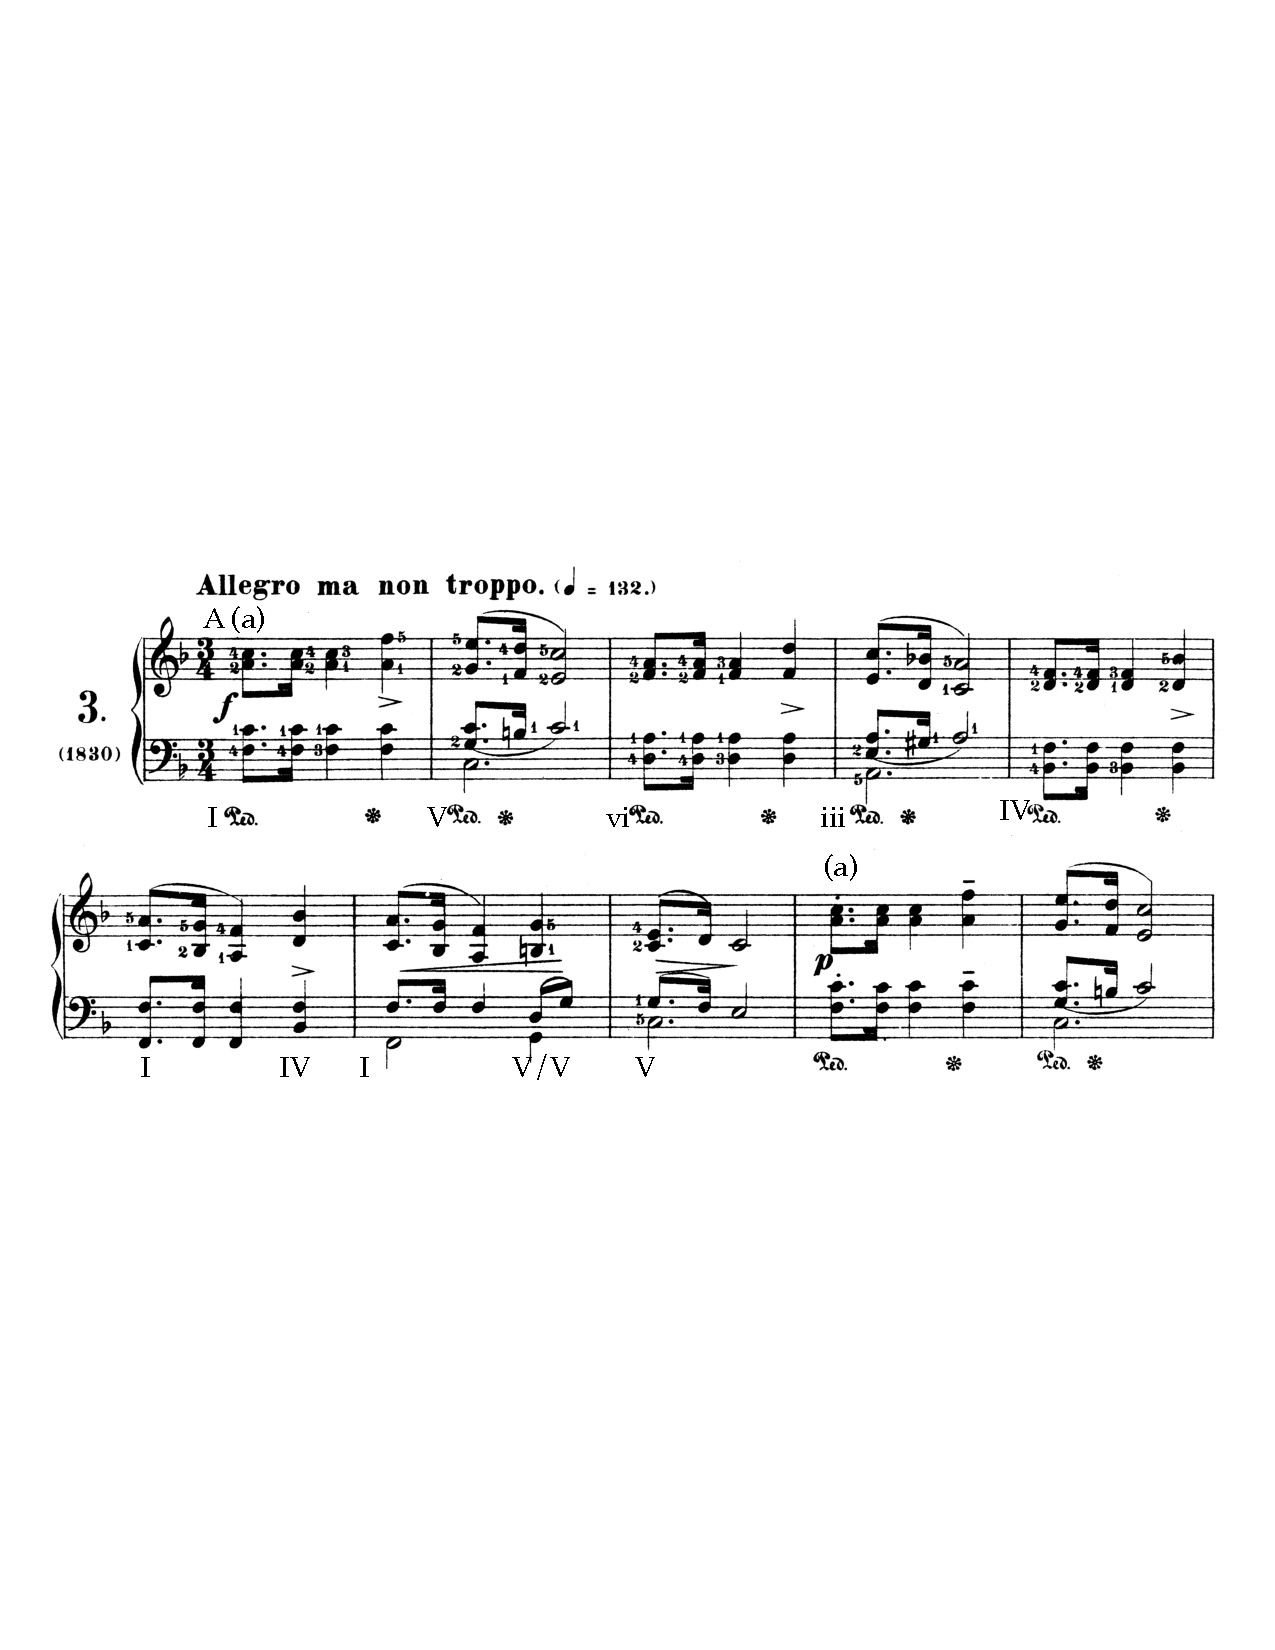
\includegraphics[width=.9\textwidth]{mazurka-first-10}
  \caption{The first ten measures of Chopin's Mazurka Op.\ 68, No.\
    3. The harmonic progression is indicated below the staff in Roman
    numerals. Sections are marked above the staff, e.g., A
    (a). Analysis by the authors. This image comes from the complete
    score published by Bote and Bock in 1880. This composition is in
    the public domain, and the score is freely available via the
    International Music Score Library Project.}
  \label{fig:mazurka-10}
\end{figure}
The harmonies are standard, in fact, they are essentially the same as
those of Pachelbel's {\em Canon}, familiar to many as ``that song
played at weddings.'' These harmonies, combined with the
rhythmic repetition suggests a further division of this and
all analogous sections into three small groupings: two two-measure
phrases, followed by a four-measure phrase.

As a performer, these harmonic, rhythmic, and structural analyses aid
in interpretation. The performer needs to decide how to emphasize or
deemphasize these demarcations with slight or overt tempo or dynamic
alterations. In a live performance, she could use physical motion to
further suggest a particular interpretation. She can choose to
emphasize long phrases, in this 
case, phrases of eight measures, or the shorter sub-phrases. Because
of the repetition of similar phrases, she may choose to emphasize the
long phrase on the first occurrence and shorter sub-phrases later on
for variety, for example. While the musical structure suggests such
possible interpretations, the performer must make these choices on
their own, and may even alter those decisions from performance to
performance.



\subsection{Archetypal performances}
\label{sec:arch-perf}


\begin{figure}[t]
  \centering
  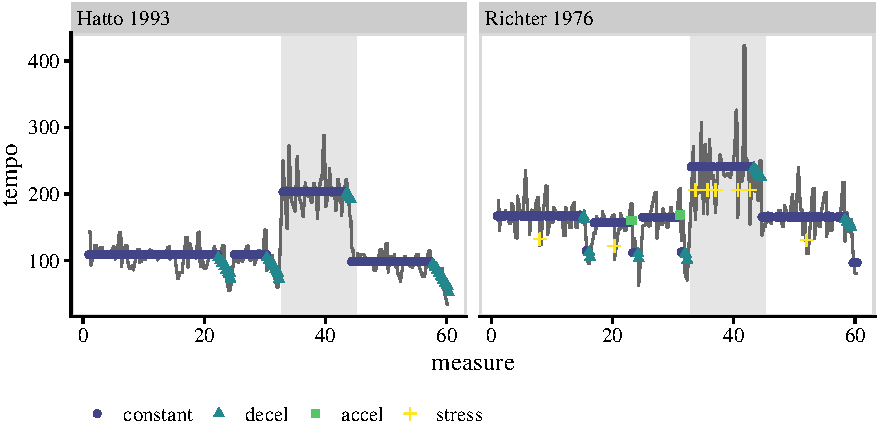
\includegraphics[width=.9\textwidth]{two-performances-1}
  \caption{Inferred performer choices for two recordings. }
  \label{fig:archetypal}
\end{figure}
Here we will carefully investigate how our model learns interpretive
decisions for three rather different performances. \autoref{fig:archetypal} shows the inferred state sequence for
recordings made by Joyce Hatto in 1993 and Sviatislav Richter in
1976. The B section is
shaded in gray to better illustrate the formal divisions discussed above.

In terms of our model, these two performers are quite different
from each other. Hatto maintains a constant tempo carefully, remaining
in state 1 with the exception of four periods of deceleration. All
four periods coincide with the most significant phrase endings: at the
end of the A section at measure 32, the end of the B section at
measure 48, at the end of the piece, and the minor transition from
$b\rightarrow a$ in the first A section (measure 24). According
to our inferred model, she never accelerates or uses the transitory
stress state.

In contrast, Richter uses all four states from our model. The short
blips of acceleration before the B section and before the
$b \rightarrow a$ transition are slightly out of place, and are
likely better labelled as ``constant'', but these state transitions
describe more severe decelerations than the model's linear
assumption would allow. Richter uses stress frequently. Some may well be
attributable to larger variance around constant tempo (picked up as
frequent stress rather than larger $\sigma^2_\epsilon$), but most
correspond to interesting note emphases, for example the second beat
of measure 20. This note is essentially a minor phrase ending, but is
also marked in the score with a {\em sforzando} (with sudden
emphasis). It's the first of two such occurrences in the piece, the
second coming four measures later on the {\em fermata}, Richter's slowest
note in the entire piece. Richter likely chooses to make this
prescribed emphasis with a sudden slow down in part because it takes
place within the context of an already loud passage, precluding the
use of extra volume.
\begin{table}[tb]
  \centering
  \caption{The estimated parameters for performances by Richter and
    Hatto.}
  \resizebox{\linewidth}{!}{%
  \begin{tabular}{@{}lrrrrrrrrrrrr@{}}
    \toprule
    & $\sigma^2_\epsilon$ & $\mu_{\textrm{tempo}}$
    & $\mu_{\textrm{acc}}$ & $\mu_{\textrm{stress}}$
    & $\sigma^2_{\textrm{tempo}}$ & $p_{11}$ & $p_{12}$ & $p_{22}$
    & $p_{31}$ & $p_{13}$ & $p_{21}$ & $p_{32}$\\
    \midrule
    Richter 1976 & 426.70 & 136.33 & -11.84 & -34.82 & 439.38
                                  & 0.85 & 0.05 & 0.74 & 0.44 & 0.02 & 0.25 & 0.17\\
    Hatto 1993 & 405.57 & 130.36 & -13.57 & -27.93 & 408.99
                                  & 0.94 & 0.03 & 0.82 & 0.36 & 0.01 &
                                                                       0.16 & 0.19\\
    Cortot 1951 & 403.71 & 182.84 & -21.43 & -45.67
    & 460.82 & 0.92 & 0.02 & 0.71 & 0.34 & 0.03 & 0.23 & 0.09\\
    \bottomrule
  \end{tabular}
}
\label{tab:two-perf-parm}
\end{table}
\autoref{tab:two-perf-parm} shows the estimated parameters for these
two performances. Richter has larger observation variance,
$\sigma^2_{\epsilon}$, slightly faster average tempo, lower
acceleration, and larger stress. He also has a larger tempo variance,
meaning that returns to state 1 can start at relatively different
tempos. On the other hand, Hatto is much more
likely to remain in states 1 or 2. These inferences are largely
consistent with the visual takeaways of \autoref{fig:archetypal}. It's
easy to see the increased variability around the constant tempo in
Richter's performance and the faster overall tempos in both the A and
B sections.
%
While these two performances are quite different from each other, they
also display similarities. Both take a faster tempo in the B
section versus the A sections. Both performers slow down at the end of
the piece, at the end of the B section, immediately preceding the B section, and at the
$b\rightarrow a$ transition.

Alfred Cortot's 1951 performance is displayed
in~\autoref{fig:cortot}. Both in terms of the parametric model we
propose, and if we simply compare the vectors of note-by-note tempos
(discussed in more detail below), this performance is an
outlier. Cortot never uses the deceleration state, and he remains in
constant tempo for the entirety of both A sections. While the model
describes his performance well, it also illustrates a deficiency of
this approach: Cortot, more than any other performer, has large
contrasts between the A and B sections. His A section is the slowest
of all 46 recordings at around 64 b.p.m., half the marked
tempo. The next slowest is Maryla Jonas's recording at around 84
b.p.m. Meanwhile, his B section is among the fastest of all the
recordings and contains the fastest individual note. Additionally,
there is stunningly little tempo variability in his A sections, but
dramatic variation in the B section coupled with frequent uses of the
acceleration and emphasis states. Taken together, Cortot's performance
may be better described by estimating our model separately on the two sections.
\begin{figure}[t]
  \centering
    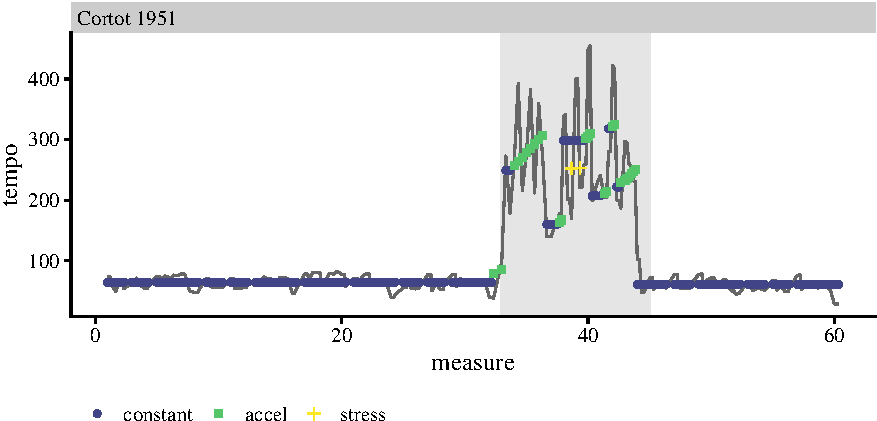
\includegraphics[width=.9\textwidth]{cortot-performance-1}
  \caption{Inferred performance choices for Alfred Cortot's 1951
    recording.}
  \label{fig:cortot}
\end{figure}



\subsection{Clustering musical performances}
\label{sec:clust-music-perf}

To better understand how all the 46 performances relate to each other,
we applied parametric clustering using the eleven-dimensional vector
of estimated parameters. Because the estimated parameters are of
different scales, have different domains, and can covary, we treat
them differentially. To calculate distances between the mean and
variance parameters, $\sigma^2_\epsilon$, $\mu_{\textrm{tempo}}$,
$\mu_{\textrm{acc}}$, $\mu_{\textrm{stress}}$, and
$\sigma^2_{\textrm{tempo}}$ we simply use Euclidean distance on each
individually. In the cases of the probabilities, we use weighted
Euclidean distance in the prior precision. For example, for
$p_{1\cdot}$, we calculate
\begin{equation}
d\left(p_{1\cdot},\ p'_{1\cdot}\right) = (p_{1\cdot}-p'_{1\cdot})^\top
  \Omega (p_{1\cdot}-p'_{1\cdot}),\quad
\textrm{where}
  \quad\Omega^{-1}_{ij} := \Sigma_{ij} :=
  \alpha_0^{-2}(\alpha_0+1)^{-1}\left(\alpha_i\alpha_0 \delta_{ij}
    - \alpha_i\alpha_j\right),
\end{equation}
is the covariance matrix of the Dirichlet distribution with
$\alpha_0=\sum_i\alpha_i$ and $\delta_{ij}$ the indicator that
$i=j$. We then standardize each individual distance matrix to have a
maximum distance of 1 and add them together so that the maximum distance
between performances is 8.


\begin{figure}[t]
  \centering
  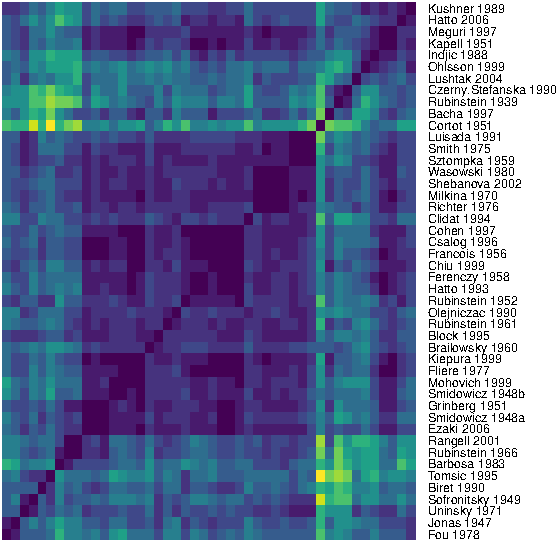
\includegraphics[width=.45\linewidth]{parametric-clusters-1}
  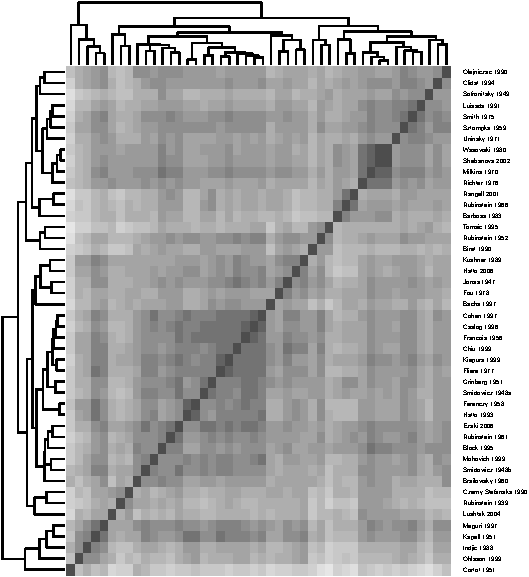
\includegraphics[width=.45\linewidth]{parametric-clusters-2}
  \caption{Distance matrix using estimated model parameters. Left: the
    matrix for all 46 parameters. Right: The same matrix with
    ``outlying'' performances removed and a dendrogram from hierarchical
    clustering.}
  \label{fig:dmats}
\end{figure}
\autoref{fig:dmats} shows the distance matrix calculated from the
estimated parameters for all 46 performances (left) and the same
matrix with ``outlying'' performances removed (right). To determine
outlying performances, we calculated the distance to the third nearest
performance. We then removed those performances that exceeded a
threshold, meaning that the nearest similar performances were ``far
away''. This screening left 25 performances. We used hierarchical
clustering on these 25 performances, trying between two and five
clusters. The remaining 21 were grouped together as ``other''. The
right panel of \autoref{fig:dmats} displays this subset along with a
dendrogram and four clusters.

\begin{figure}[t]
  \centering
  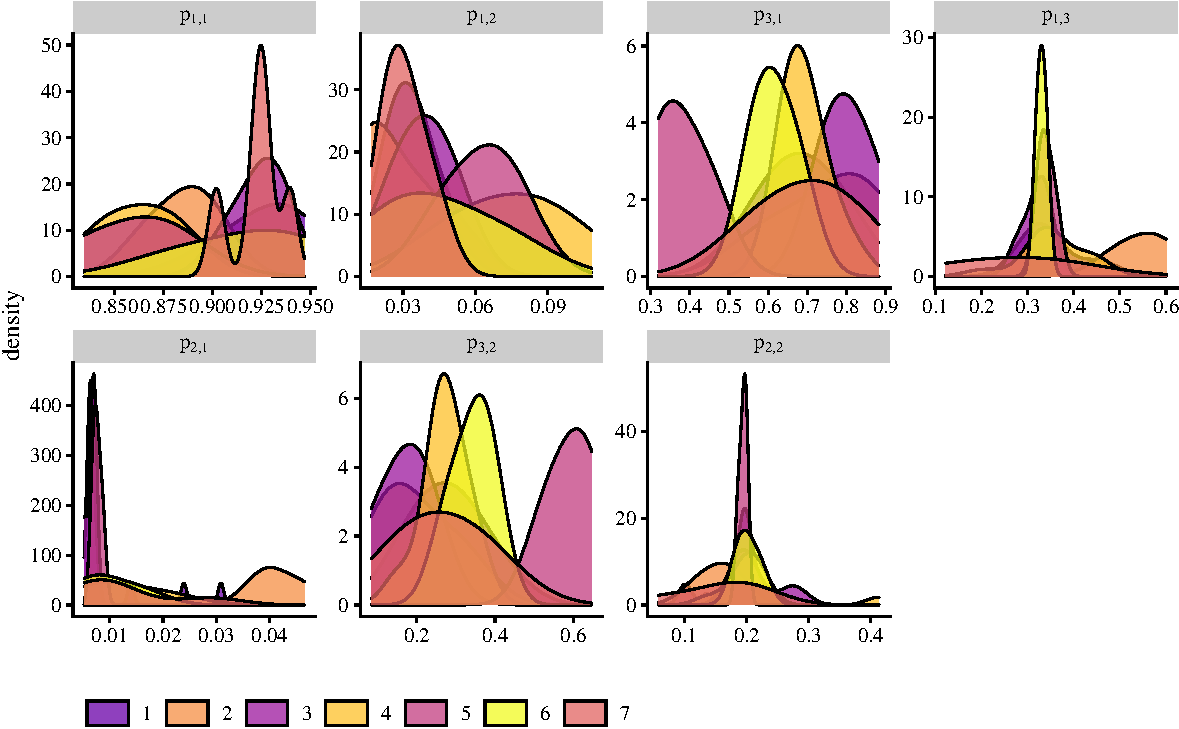
\includegraphics[width=.9\linewidth]{clust-densities-sub2-1}
  \caption{Cluster densities for Markov transition probabilities.}
  \label{fig:clust-density-tp}
\end{figure}
\begin{figure}[t]
  \centering
  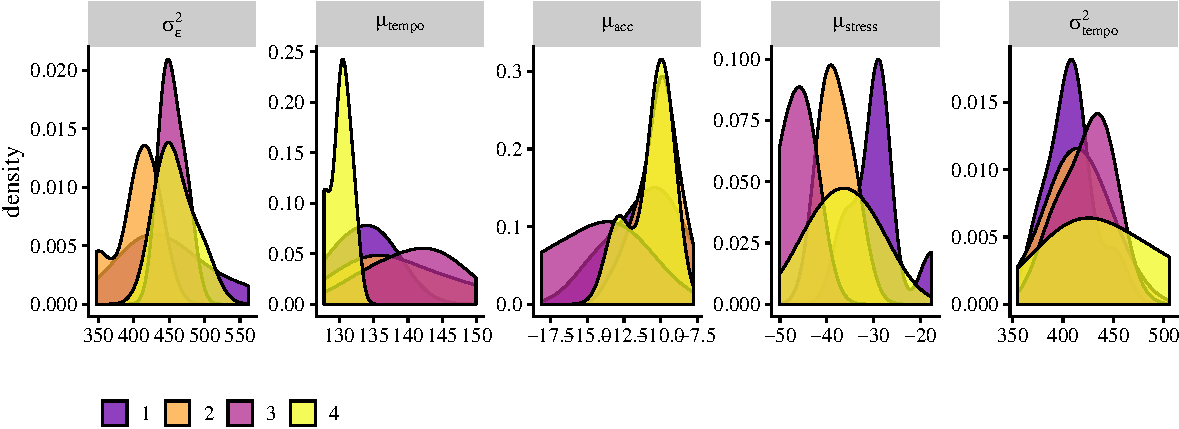
\includegraphics[width=.9\linewidth]{clust-densities-sub1-1}
  \caption{Cluster densities for mean and variance parameters.}
  \label{fig:clust-density-mv}
\end{figure}
The first cluster corresponds to performances which are reasonably
staid. The emphasis state is rarely visited with the performer tending
to stay in the constant tempo state with periods of slowing down at
the ends of phrases. Acceleration is never used. Such state
preferences are clearly inferred by the model as shown in the
top row of \autoref{fig:clust-density-tp}. Furthermore, these
performances have relatively low average tempos, and not much
difference between the A and B sections. Joyce Hatto's performance
shown in \autoref{fig:archetypal} is typical of this cluster.

Recordings in the second
cluster tend to transition quickly between states, especially constant
tempo and slowing down accompanied by frequent transitory
emphases. The probability of remaining in state 1 is the lowest while
the probability of entering state 2 from state 1 is 
the highest. The acceleration state is rarely visited. Four of
the most similar performances are in this cluster, shown in
\autoref{fig:similar}, along with Richter's 1976 recording.
\begin{figure}[t]
  \centering
  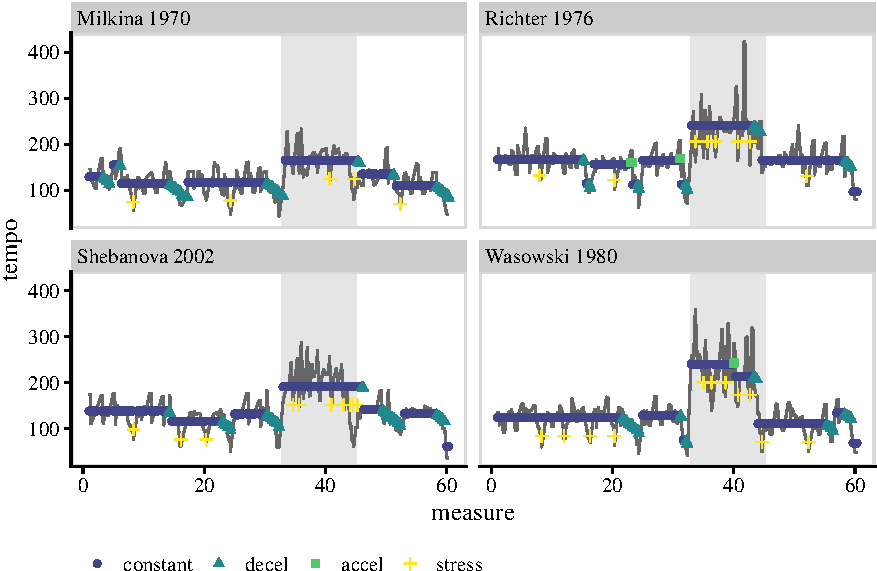
\includegraphics[width=.9\linewidth]{similar-perfs-1}
  \caption{Four similar performances, all in the second cluster.}
  \label{fig:similar}
\end{figure}

Cluster three is somewhat like cluster one in that performers tend to
stay in state 1 for long periods of time, but they transition more
quickly from state 3 back to state 1. They also use state 4 frequently
whereas cluster one
did not. They tend to have very large tempo
contrasts between the A and B sections.
Cluster four has both faster average tempos and more variability from one period of
constant tempo to the next. State 4 is rare, instead using constant tempo 
states that persist for small amounts of time to reflect note
emphases.

% \begin{figure}[t]
%   \centering
%   \includegraphics[width=.45\linewidth]{raw-data-clusters-1}
%   \caption{Distance matrix and dendrogram calculated using the
%     note-by-note tempo vector for each recording.}
%   \label{fig:raw-data-clusters}
% \end{figure}
Comparing our clusters to those we would find from simply clustering
the distances between note-by-note tempo vectors reveals a number of
differences (see the Supplement for the distance matrix calculated in
this way). The four recordings in \autoref{fig:similar} would be
spread across three different clusters, for example, as would our
cluster one. On the other hand, both metrics see Cortot's recording as a
strong outlier, and clustering by tempo vectors often (somewhat
miraculously) groups recordings by the same pianist together: both
recordings by Smidowicz, three of the four recordings by Rubinstein,
both recordings by Hatto.
\begin{figure}[t]
  \centering
  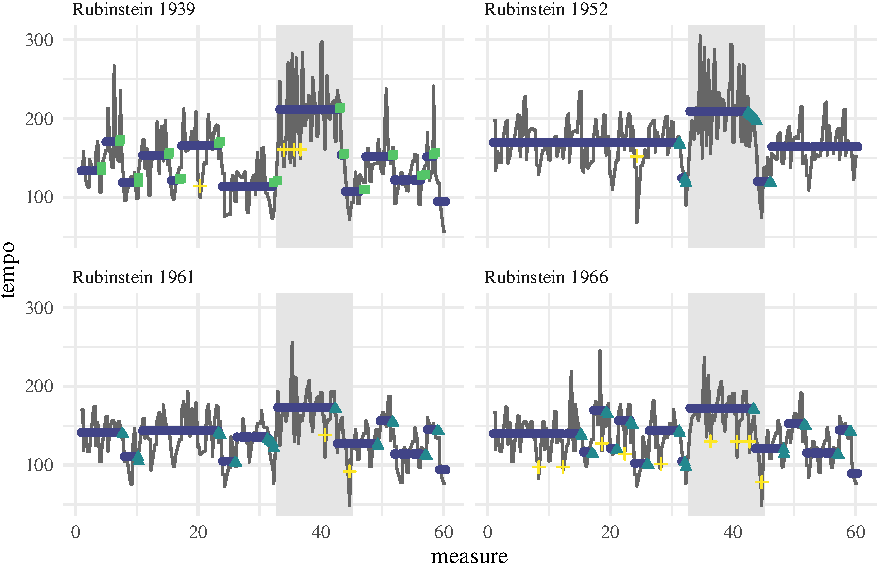
\includegraphics[width=.9\linewidth]{rubinstein-perfs-1}
  \caption{The four recordings by Arthur Rubinstein. Our clustering
    puts the 1952 and 1961 recordings in clusters one and two while
    leaving the others out. Clustering by tempo vector separates 1952
    from the other three.}
  \label{fig:rubinstein}
\end{figure}
\autoref{fig:rubinstein} shows all four Rubinstein recordings. The
1939 recording is rather odd in that the measures 24--32 are so slow
relative to the rest of the A section. The variability in the 1966
recording nearly obscures the contrast between the B section and the
surrounding A sections. These two recordings are nonetheless clustered
together by the tempo vectors. Our method on the other hand, puts both
in the ``other'' grouping. The estimated parameters for these four
performances are shown in the bottom half of
\autoref{tab:similar-different-perf}. The top half shows the
parameters for the four similar performances in
\autoref{fig:similar}. There is much larger variability across
Rubinstein's recordings, as we would expect.
\begin{table}[tb]
  \centering
  \caption{The estimated parameters for the four similar performances
    in Cluster Two and those for all four by Arthur Rubinstein.
    \label{tab:similar-different-perf}}
  \resizebox{\linewidth}{!}{%
  \begin{tabular}{@{}lrrrrrrrrrrrr@{}}
    \toprule
    & $\sigma^2_\epsilon$ & $\mu_{\textrm{tempo}}$
    & $\mu_{\textrm{acc}}$ & $\mu_{\textrm{stress}}$
    & $\sigma^2_{\textrm{tempo}}$ & $p_{11}$ & $p_{12}$ & $p_{22}$
    & $p_{31}$ & $p_{13}$ & $p_{21}$ & $p_{32}$\\
    \midrule
    Wasowski 1980 & 414.99 & 132.00 & -10.00 & -40.00
    & 425.00 & 0.85 & 0.05 & 0.67 & 0.34 & 0.02 & 0.26 & 0.20\\
    Shebanova 2002 & 439.98 & 132.00 & -10.00 & -40.00
    & 400.02 & 0.85 & 0.05 & 0.67 & 0.33 & 0.02 & 0.27 & 0.20\\
    Luisada 1991 & 494.33 & 127.80 & -10.24 & -32.56
    & 411.63 & 0.84 & 0.10 & 0.71 & 0.35 & 0.01 & 0.26 & 0.19\\
    Milkina 1970 & 435.25 & 136.38 & -9.68 & -40.02 & 400.01
                                  & 0.87 & 0.05 & 0.68 & 0.33 & 0.02 &
                                                                       0.26 & 0.21\\
    \midrule
    Rubinstein 1939 & 520.32 & 145.26 & -7.89 & -50.82
    & 345.64 & 0.89 & 0.02 & 0.83 & 0.56 & 0.05 & 0.13 & 0.16\\
    Rubinstein 1952 & 481.13 & 128.13 & -7.76 & -17.59
    & 409.30 & 0.93 & 0.04 & 0.68 & 0.32 & 0.01 & 0.28 & 0.19\\
    Rubinstein 1961 & 434.23 & 139.17 & -8.34 & -35.08
    & 355.00 & 0.90 & 0.06 & 0.56 & 0.46 & 0.01 & 0.41 & 0.19\\
    Rubinstein 1966 & 380.95 & 127.24 & -8.80 & -42.28
    & 473.69 & 0.87 & 0.07 & 0.36 & 0.34 & 0.01 & 0.61 & 0.20\\
    \bottomrule
  \end{tabular}
  }
\end{table}


\subsection{Alternative smoothers}
\label{sec:altern-smooth}

Our model is just one type of smoothing one could imagine using to
find low-dimensional structure for the vector of note-by-note
tempos. Alternative statistical techniques are common, and examining
how they compare with our method helps to illuminate some of its
benefits. The most obvious alternative is to use smoothing
splines~\citep{CravenWahba1978,Wahba1990} though total-variation
denoising or trend filtering \citep{KimKoh2009,Tibshirani2014} are
other reasonable alternatives.
These statistical techniques perform smoothing by encouraging small
changes in derivatives (smoothing splines) or bounded total variation
(trend filtering). 
But musical performances do not conform to these assumptions because tempo interpretations rely on the juxtaposition of local smoothness
with sudden changes and emphases to create listener interest. It is
exactly the parts of a performance that are poorly described by
statistical smoothers that render a performance
interesting. Furthermore, many of these
inflections are notated by the 
composer or are implicit in performance practice developed over
centuries of musical expressivity. Consequently, smoothing that
incorporates domain knowledge leads to better statistical and
empirical results.
\begin{figure}[t]
  \centering
  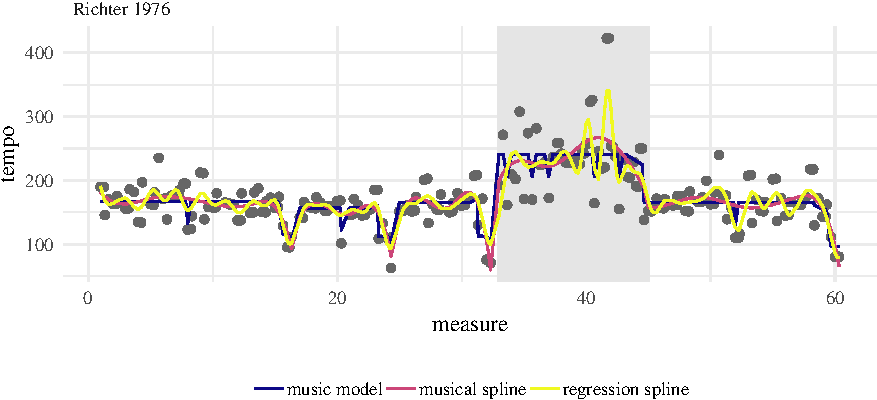
\includegraphics[width=.9\linewidth]{alternative-smoothers-1}
  \caption{Smoothing with splines and musical models}
  \label{fig:splines}
\end{figure}

\autoref{fig:splines}
shows the note-by-note tempo of Richter's 1976 recording. Splines with
equally spaced knots are shown in yellow. We use generalized cross
validation~\citep{GolubHeath1979} to select the number of knots (one
knot per measure). The red line shows a regression spline fewer knots,
but whose locations were chosen
manually
to coincide with the musical phrase endings discussed in
\autoref{sec:musical-analysis}. Knots at phrase endings were
duplicated up to four times to allow for discontinuities. The blue line 
shows the estimated smooth tempo from our model (the same as in
\autoref{fig:archetypal}). The regression spline with
equally spaced knots undersmooths in constant tempo areas in an
attempt to capture sudden emphases and dramatic changes in others. The spline
with informed knot choice does much better, picking up the periods of
deceleration at the ends of phrases. Our model learns these behaviors
on its own while also capturing individual emphases that are missed in
the musical analysis but are idiosyncratic to Richter's playing. It is
also more parsimonious to musical interpretation, inferring constant
tempo periods rather than resulting in smoothly varying tempos in
stable periods.%, such as measures 1--16.

\subsection{Problems with the model and estimation}
\label{sec:problems-with-model}

While our model of musical decision making yields interesting insights
into performance practice most of the time, it also suffers from some
deficiencies. As discussed above in reference to Alfred Cortot's
recording, the assumption that all parameters are stable over the
entire piece may not always be accurate. The $\mu_{\textrm{tempo}}$
parameter especially, should be estimated separately in different
sections. This problem will only be compounded in more complex music
with many contrasting sections. A related issue is the current form
for the slowing down and speeding up sections. Our model assumes that
both occur linearly, with a constant decrease of $\mu_{\textrm{acc}}$
b.p.m. An ability to slow increasingly as one remains in the state may
improve the model fit.

There is nothing intrinsic to the model which forces states 2,
3, or 4 to always go in the correct direction. If for example,
$\mu_{\textrm{acc}}$ is small in magnitude relative to
$\sigma^2_{\textrm{acc}}$, an acceleration could be learned as time
spent in state 2 but with large positive errors. For this piece, the
penalties help to avoid such occurrences, but this aspect of the
Gaussian state-space model could be improved by enforcing non-Gaussian
behavior. Or course, such constraints would complicate likelihood
evaluation since the Kalman filter could no longer be used. Relatedly,
our model produced objectively incorrect inferences on two performances
\begin{figure}[t]
  \centering
  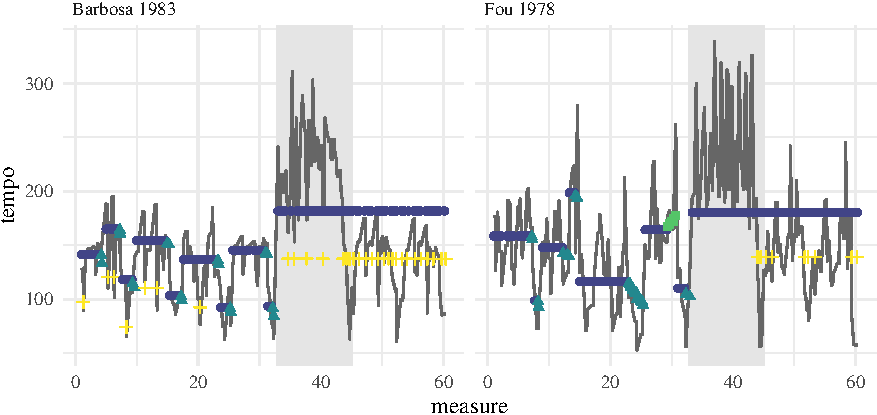
\includegraphics[width=.9\linewidth]{bad-model-1}
  \caption{Estimation errors on two performances.}
  \label{fig:bad-model}
\end{figure}
(\autoref{fig:bad-model}). Here, the estimated
path failed to transition to state 1 at the
recapitulation of the A section. In both cases, the resulting path
stands out dramatically, remaining in the much faster constant tempo
state from the B section with overly frequent emphases. Both of these
performances are quite volatile, making estimation difficult, and were clustered as ``other''. 

% One issue in our model that the effect of states two and three can be flipped. If $\tau_t$ is small enough, and $\sigma_4^2$ and $\sigma_2^2$ are large enough, it would be possible to get a negative number for the acceleration term when in state 2 or a positive number when in state three and still get a reasonably high likelihood. This could be fixed by adding a constraint on the ratio of the $\tau_t$ and $\sigma$'s 2 and 4.

\section{Discussion}
\label{sec:discussion}


Musical interpretation is the most important factor 
in determining whether or not concertgoers enjoy a classical performance. Every
performance includes mistakes---intonation issues, a lost note, an
unpleasant sound---but these are all easily forgotten (or unnoticed) when a performer
engages her audience, imbuing a piece with novel emotional content
beyond the vague instructions inscribed on the printed page. While music teachers use
imagery or heuristic guidelines to motivate interpretive decisions, combining these
vague instructions to create a convincing performance remains the domain
of the performer, subject to the whims of the moment, technical
fluency, and taste.

In this paper, we develop a statistical model for tempo to elucidate performance
decisions from classical music recordings. We present an algorithm for
performing likelihood inference, estimate our model using a large
collection of recordings of the same composition, and demonstrate how
the model is able to recover performer intentions, and how they relate
to standard musical analysis. While our methods perform well, our
analysis reveals a number of avenues for future work an
improvement. For the piano, apart from tempo decisions, the performer
can also control dynamics differentially. Similar techniques to those
employed here could be used to describe levels of loudness, and
creating a model that combined both is desirable. Pianists have
relatively few variables under their control for interpretation:
tempo, dynamics, and pedalling. On the other had, string players have
many more. Bowing decisions, fingerings, vibrato, broken chords are
all important tools which are difficult to learn from a recording, let
alone describe with a simple statistical model. Significant work would
be required to generalize our techniques to more detailed
interpretative analysis. On the other hand, focusing simply on tempo
can be useful with solo performances or with larger
ensembles. Examining more complex genres---sonatas, string quartets,
symphonies---would also be interesting for future work.

Another avenue we wish to pursue in the future is to examine how our
model's implications may be useful for teaching students. Can we
estimate it quickly to provide immediate feedback to novice pianists?
In this paper, we used a dataset in which the note-by-note tempos were
annotated by experienced musicians. Combining our model with existing
approaches to solving the note-score alignment problem
\citep{LangFreitas2005,Raphael2002,DannenbergRaphael2006}, perhaps to
their benefit would be the first step. Together, this could produce an
immediate graphical representation that students and teachers could
use to evaluate and improve their practice.

\bigskip
\begin{center}
{\large\bf SUPPLEMENTARY MATERIAL}
\end{center}

\begin{description}

\item[R-package ``dpf'':] R-package containing code to perform the
  methods described in the article. The package also contains all data
  sets used as examples in the article. (GNU zipped tar, also on
  Github)
  
\item[Source code:] Additional R code necessary to reproduce all
  analyses and graphics. (GNU zipped tar, unblinded)

\item[Appendix:] Supplement with additional graphics for all clusters
  and analysis of all 46 recordings. (PDF)

\end{description}


\clearpage



\bibliographystyle{mybibsty}
\bibliography{chopinrefs}

\appendix

\hypertarget{algorithms}{%
\section{Algorithms}\label{algorithms}}

For completeness, we include here concise descriptions of the Kalman
filter and smoother we employ as inputs to our main algorithm. The
filter is given in \autoref{alg:kalman}.

\begin{algorithm}
  \caption{Kalman filter: estimate $x_i$ conditional on
    $\{y_j\}_{j=1}^i$, for all $i=1,\ldots,n$ and calculate the log likelihood
    for $\theta$\label{alg:kalman}}
  \begin{algorithmic}
    \STATE {\bf Input:} $Y$, $x_0$, $P_0$, $d,\ T,\ c,\ Z,$ and $G$
    \STATE $\ell(\theta) \leftarrow 0$ \COMMENT{Initialize the log-likelihood}
    \FOR{$i=1$ to  $n$}
    \STATE $\begin{aligned}\varx_{i}
      &\leftarrow d + T x_{i-1|i-1}, & P_i &\leftarrow Q + T P_{i-1|i-1}
      T^\top\end{aligned}$ \COMMENT{Predict current state}
    \STATE $\begin{aligned}\widetilde{y}_i
      &\leftarrow c + Z \varx_i, & F_i &\leftarrow G + Z P_i
      Z^\top\end{aligned}$ \COMMENT{Predict current observation}
    \STATE $\begin{aligned}v_i&\leftarrow y_i-\widetilde{y}_i& K_i&
      \leftarrow P_i Z^\top F^{-1}\end{aligned}$ \COMMENT{Forecast error and 
    Kalman gain}
    \STATE $\begin{aligned} x_{i|i}
      &\leftarrow \varx_i + K_i v_i, & P_{i|i} &\leftarrow P_i - P_iZ^\top
      K_i\end{aligned}$ \COMMENT{Update}
    \STATE $\ell(\theta) = \ell(\theta) -v_i^\top F^{-1}v_i - \log(|F_i|)$
    \ENDFOR
    \RETURN $\widetilde{Y}=\{\widetilde{y}_i\}_{i=1}^n,\ \varx=\{\varx_i\}_{i=1}^n,\
    \widetilde{X}=\{x_{i|i}\}_{i=1}^n,\ P=\{P_i\}_{i=1}^n,\
    \widetilde{P}=\{P_{i|i}\}_{i=1}^n,\ \ell(\theta)$
  \end{algorithmic}
\end{algorithm}

To incorporate all future observations into these estimates, the Kalman
smoother is required. There are many different smoother algorithms
tailored for different applications. \autoref{alg:kalman-smoother}, due
to \citet{RauchStriebel1965}, is often referred to as the classical
fixed-interval smoother \citep{AndersonMoore1979}. It produces only the
unconditional expectations of the hidden state
\(\hat{x}_i=\Expect{x_i\given y_1,\ldots,y_n}\) for the sake of
computational speed. This version is more appropriate for inference in
the type of switching models we discuss in the manuscript.

\begin{algorithm}
  \caption{Kalman smoother (Rauch-Tung-Striebel): estimate $\hat{X}$ conditional on
    $Y$\label{alg:kalman-smoother}} 
  \begin{algorithmic}
    \STATE {\bf Input:} $\varx$, $\widetilde{X}$, $P$, $\widetilde{P}$,
    $T,$ $c$, $Z$.
    \STATE $t=n$,
    \STATE $\hat{x}_{n}\leftarrow \widetilde{x}_n$, 
    \WHILE{$t>1$}
    \STATE $\hat{y}_i \leftarrow c + Z\hat{x}_i,$
    \COMMENT{Predict observation vector}
    \STATE $\begin{aligned} e &\leftarrow \hat{x}_i -
      \varx_i, & V &\leftarrow P_i^{-1}\end{aligned}$,
    \STATE $t\leftarrow i-1$, \COMMENT{Increment}
    \STATE $\hat{x}_i = \widetilde{x}_i + \widetilde{P}_i T Ve $ 
    \ENDWHILE
    \RETURN $\widehat{Y}=\{\hat{y}_i\}_{i=1}^n, \hat{X}=\{\hat{x}_i\}_{i=1}^n$
  \end{algorithmic}
\end{algorithm}

\hypertarget{distance-matrix-from-raw-data}{%
\section{Distance matrix from raw
data}\label{distance-matrix-from-raw-data}}

In \autoref{sec:clust-music-perf} of the manuscript, we present results
for clustering performances using the low-dimensional vector of
performance specific parameters learned for our model. An alternative
approach is to simply use the raw data, in this case, 231 individual
note-by-note instantaneous speeds measured in beats per minute. In
\autoref{fig:raw-data-clusters} we show the result of this analysis. A
comparison between this clustering and that given by our model is
discussed in some detail in the manuscript.

\begin{figure}[b]

{\centering \includegraphics[width=3in,height=3in]{gfx/raw-data-clusters-1} 

}

\caption{This figure presents a heatmap and hierarchical clustering based only on the note-by-note onset timings for each of the 46 recordings.}\label{fig:raw-data-clusters}
\end{figure}

\hypertarget{plotting-performances}{%
\section{Plotting performances}\label{plotting-performances}}

In \autoref{sec:clust-music-perf} discussed 4 distinct clusters of the
46 performances as well as an ``other'' category of relatively unique
interpretations. Figures \ref{fig:clust-1} to \ref{fig:clust-other}
display the note-by-note tempos along with the inferred interpretive
decisions for all performances by clustering. Here we include some of
the discussion of these clusters from the main text to clarify the
figures.

The first cluster (\autoref{fig:clust-1}) corresponds to performances
which are reasonably staid. The emphasis state is rarely visited with
the performer tending to stay in the constant tempo state with periods
of slowing down at the ends of phrases. Acceleration is never used. Such
state preferences are clearly inferred by the model as shown in, e.g.,
the top row of \autoref{fig:clust-density-tp}. Furthermore, these
performances have relatively low average tempos, and not much difference
between the A and B sections.

\begin{figure}

{\centering 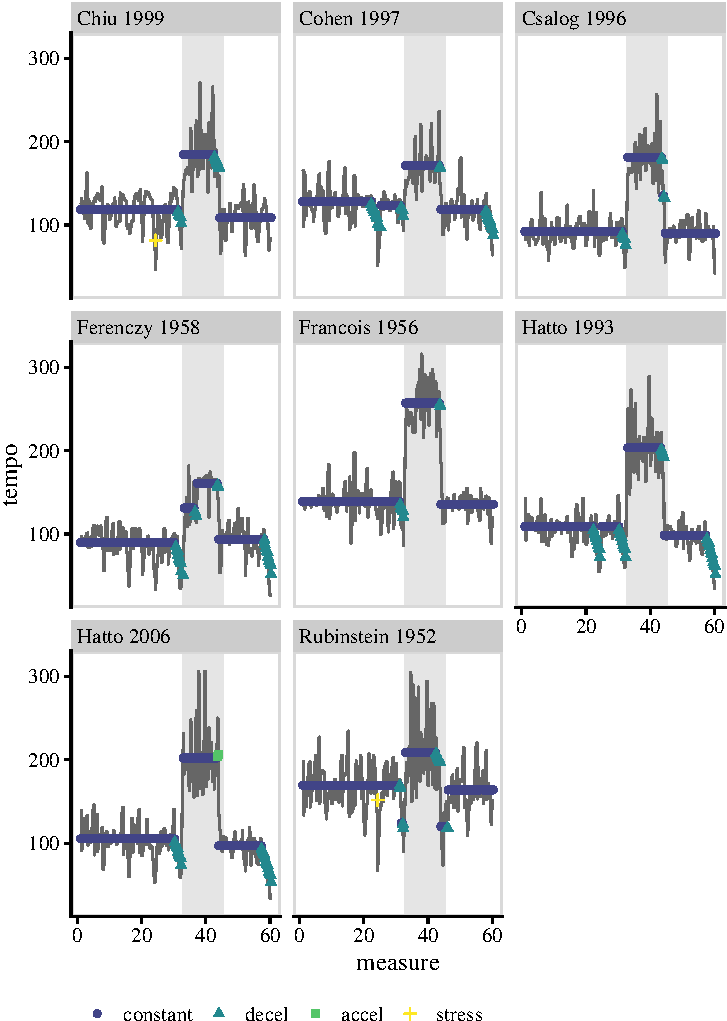
\includegraphics{gfx/clust-1-1} 

}

\caption{Performances in the first cluster.}\label{fig:clust-1}
\end{figure}

Recordings in the second cluster (\autoref{fig:clust-2}) tend to
transition quickly between states, especially constant tempo and slowing
down accompanied by frequent transitory emphases. The probability of
remaining in state 1 is the lowest for this cluster while the
probability of entering state 2 from state 1 is the highest. The
acceleration state is visited only rarely.

\begin{figure}

{\centering 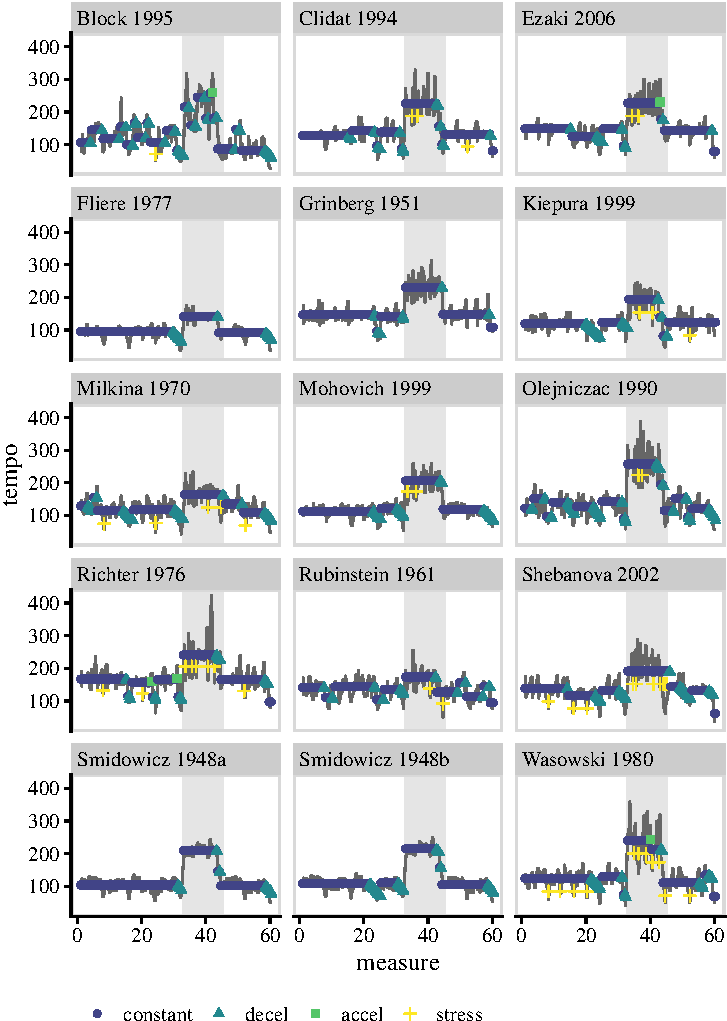
\includegraphics{gfx/clust-2-1} 

}

\caption{Performances in the second cluster.}\label{fig:clust-2}
\end{figure}

Cluster three (\autoref{fig:clust-3}) is somewhat like cluster one in
that performers tend to stay in state 1 for long periods of time, but
they transition more quickly from state 3 back to state 1. They also use
state 4 frequently whereas cluster one did not. They also tend to have
very large tempo contrasts between the A and B sections.

\begin{figure}

{\centering 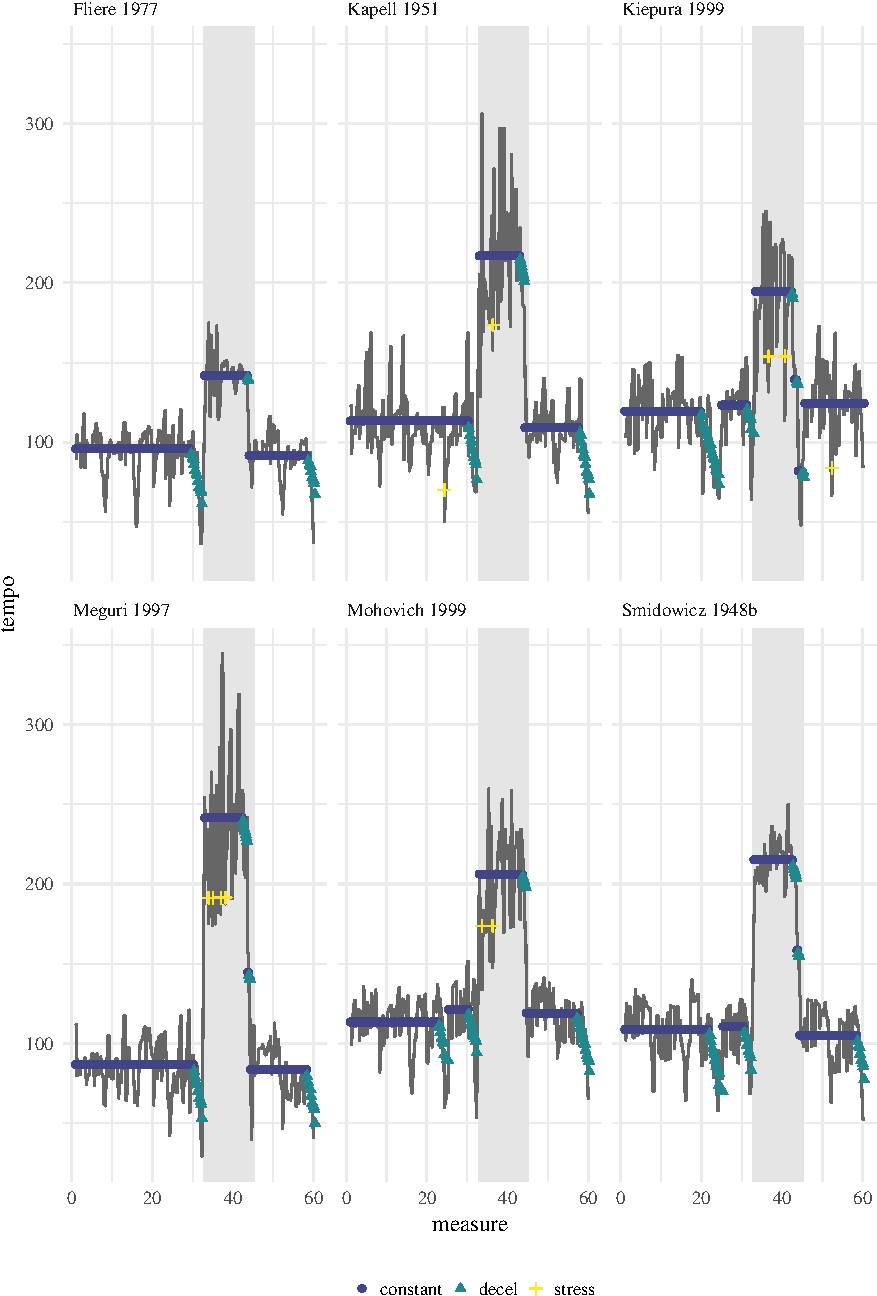
\includegraphics{gfx/clust-3-1} 

}

\caption{Performances in the third cluster.}\label{fig:clust-3}
\end{figure}

Cluster four (\autoref{fig:clust-4}) has both faster average tempos and
more variability from one period of constant tempo to the next. State 4
is rare, with fast constant tempo changes that persist for small amounts
of time tending to reflect note emphases.

\begin{figure}

{\centering 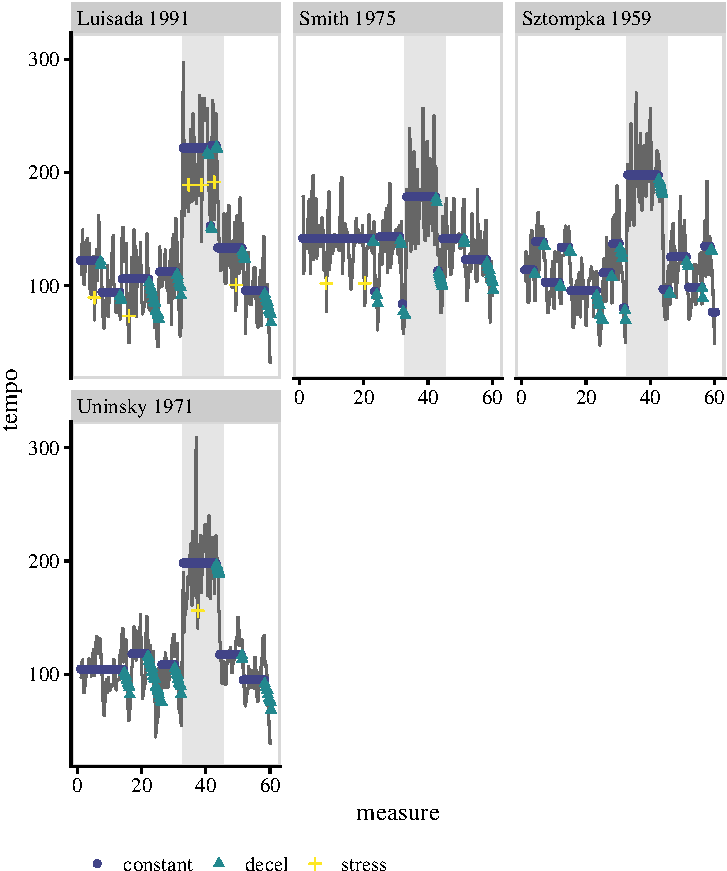
\includegraphics{gfx/clust-4-1} 

}

\caption{Performances in the fourth cluster.}\label{fig:clust-4}
\end{figure}

The remaining performances are relatively different from all other
performances (\autoref{fig:clust-other}. If the distance to the third
closest performances exceeded 0.35, then the performance was grouped
with ``other''. Essentially, these recordings had at most one similar
recording while the four other clusters contained at least 4.

\begin{figure}

{\centering 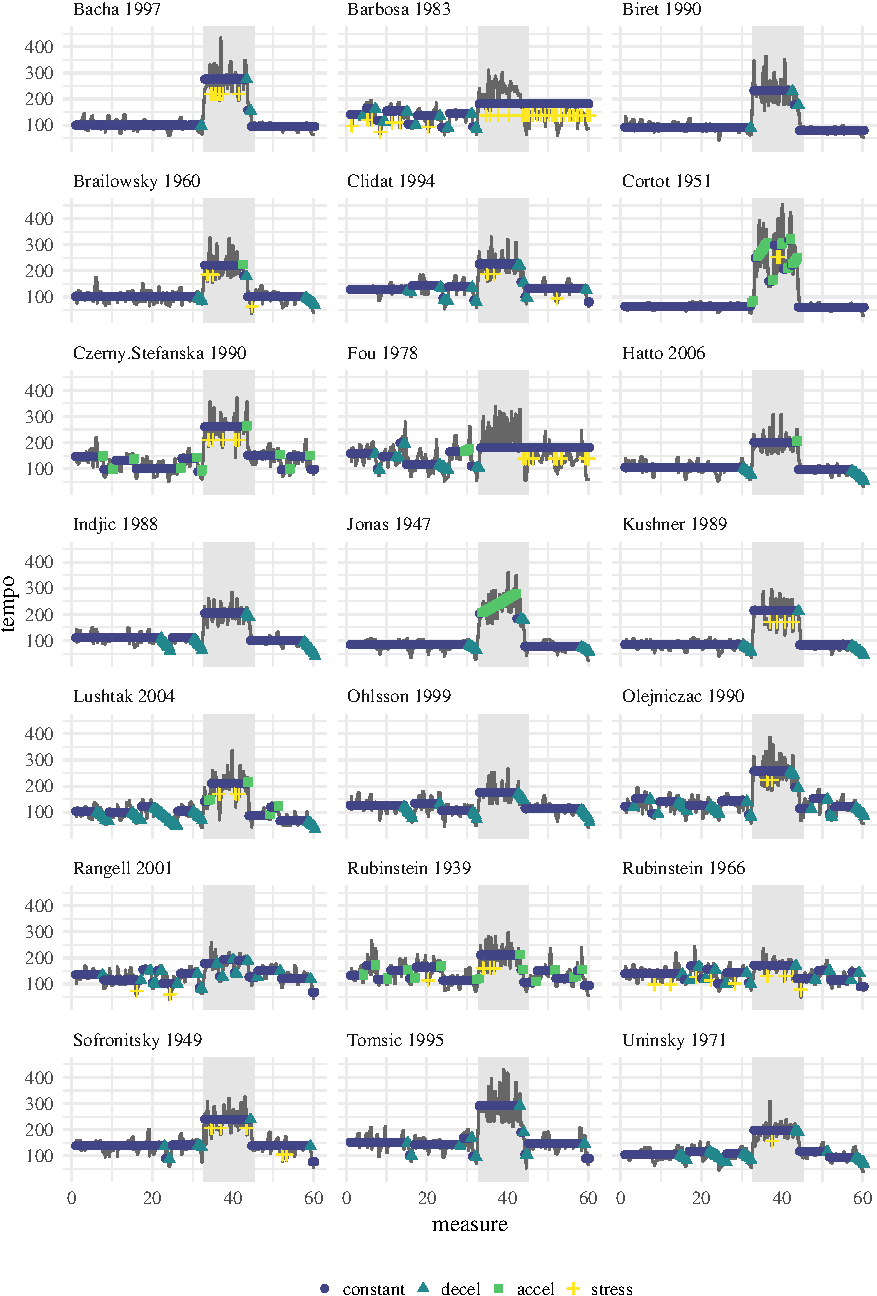
\includegraphics{gfx/clust-other-1} 

}

\caption{Performances in the ``other'' cluster.}\label{fig:clust-other}
\end{figure}



\end{document}
